\section{Introduction to Power Semiconductor Devices}
\title[Introduction to power semiconductor devices]{Introduction to power semiconductor devices}  

\subsection{Power diodes}

\begin{frame}[plain]
    \titlepage
\end{frame}

\begin{frame}{\textbf{Normal vs Power Semiconductor Devices: Key Differences}}
    \textbf{1. Physical Design:}
    \begin{itemize}
        \item \textbf{Normal Devices:} Small device areas, thin active regions for fast operation.
        \item \textbf{Power Devices:} Large device areas, thick drift regions to support high voltages; trade-off between speed and ruggedness.
    \end{itemize}

    \textbf{2. Key Parameters:}
    \begin{itemize}
        \item \textbf{Normal Devices:} Optimize \textit{speed}, \textit{gain}, \textit{integration density}.
        \item \textbf{Power Devices:} Optimize \textit{breakdown voltage}, \textit{on-resistance}, \textit{thermal management}.
    \end{itemize}

    \textbf{3. Material and Fabrication:}
    \begin{itemize}
        \item \textbf{Normal Devices:} Primarily Silicon (Si).
        \item \textbf{Power Devices:} Silicon (Si), but also wide bandgap materials like Silicon Carbide (SiC) and Gallium Nitride (GaN) for superior performance.
    \end{itemize}

    \textbf{4. Examples:}
    \begin{itemize}
        \item \textbf{Normal Devices:} CMOS transistors, Bipolar Junction Transistors (BJTs).
        \item \textbf{Power Devices:} MOSFETs, IGBTs, Diodes (Schottky, PIN), SiC MOSFETs, GaN HEMTs.
    \end{itemize}

    \vspace{0.3cm}
    \textbf{Summary:} \\
    \textit{While normal semiconductors are optimized for information processing, power semiconductors are engineered for robust control of large electrical energy flows.}
\end{frame}


%%%%%%%%%%%%%%%%%%%%%%%%%%%%%%%%%%%%%%%%%%%%%%%%%%%%%%%%%%%%%
%% Conceptual idea of power semiconductor devices physics %%
%%%%%%%%%%%%%%%%%%%%%%%%%%%%%%%%%%%%%%%%%%%%%%%%%%%%%%%%%%%%%
\begin{frame}
	\frametitle{Conceptual idea of a power semiconductor devices physics}
    \textbf{1. Charge Carriers:} 
    \begin{itemize}
        \item Power devices rely on the transport of \textbf{electrons} and \textbf{holes}.
        \item Key mechanisms: \textbf{drift} (due to electric fields) and \textbf{diffusion} (due to concentration gradients).
    \end{itemize}

    \textbf{2. Energy Bands and Junctions:}
    \begin{itemize}
        \item Junctions (e.g., p-n junctions, Schottky barriers) control carrier flow.
        \item Band bending creates potential barriers essential for device blocking and switching behavior.
    \end{itemize}

    \textbf{3. Electric Field Distribution:}
    \begin{itemize}
        \item High electric fields are engineered to manage breakdown and switching.
        \item \textbf{Critical electric field} (\( E_{crit} \)) defines breakdown limits.
    \end{itemize}
\end{frame}


\begin{frame}
	\frametitle{Conceptual idea of a power semiconductor devices physics cond.. }
\textbf{4. Key Physical Processes:}
\begin{itemize}
    \item \textbf{Avalanche Multiplication:} Carrier generation at high fields.
    \item \textbf{Recombination-Generation:} Determines carrier lifetimes.
    \item \textbf{Tunneling:} Important in very high field conditions (Zener breakdown).
\end{itemize}

\textbf{5. Device Performance Metrics:}
\begin{itemize}
    \item \textbf{Blocking Voltage:} Ability to withstand high reverse voltages.
    \item \textbf{On-State Resistance:} Determines conduction losses.
    \item \textbf{Switching Speed:} Influenced by carrier lifetimes and device capacitances.
\end{itemize}

\textbf{Summary:} \\
\textit{Power semiconductor devices are engineered by carefully controlling material properties, doping profiles, junction designs, and carrier dynamics to optimize switching behavior, conduction losses, and voltage handling capabilities.}
\end{frame}

\begin{frame}
	\frametitle{Classification of types of power semiconductor devices}
    \textbf{Based on number of terminals:}
    \begin{columns}
        \column{0.35\textwidth}
        \begin{itemize}
            \item \textbf{Two-terminal devices:}
            \begin{itemize}
                \item Diodes (e.g., Schottky, Zener, and standard rectifier diodes).
            \end{itemize}
            \item \textbf{Three-terminal devices:}
            \begin{itemize}
                \item Insulated Gate Bipolar Transistor (IGBT).
                \item Thyristors (SCRs).
            \end{itemize}
            \item \textbf{Four-terminal devices:}
            \begin{itemize}
                \item IGBT with Kelvin connection.
                \item Cascode structures (e.g., GaN HEMT with a low-voltage MOSFET).
            \end{itemize}
        \end{itemize}

        \column{0.65\textwidth}
        \begin{figure}
            \centering
            \label{fig:Classification_based_on_number_of_terminals}
            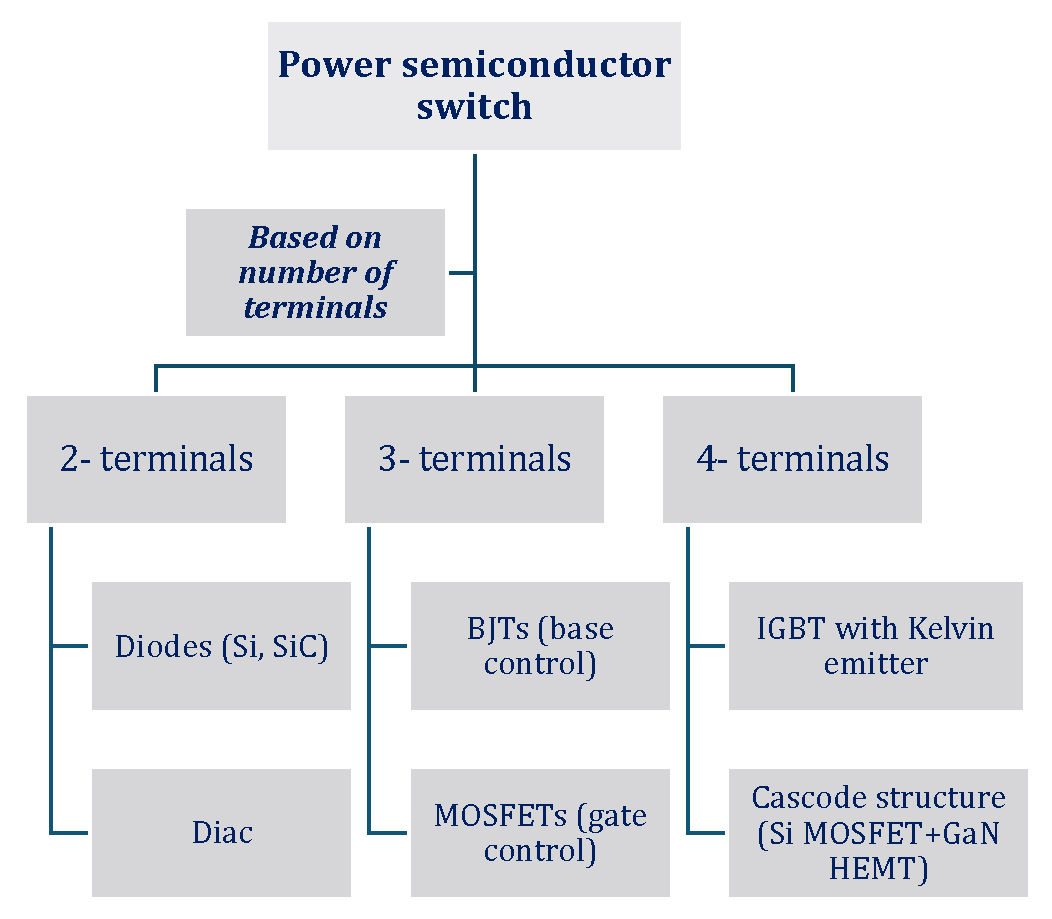
\includegraphics[scale=0.35]{fig/lec04/classification_of_device_1.eps}
            \caption{Classification of power semiconductor devices based on number of terminals.}
        \end{figure}
    \end{columns}
\end{frame}


\begin{frame}
	\frametitle{Classification of types of power semiconductor devices}
    \textbf{Based on number of layser/junctions:}
    \begin{columns}
        \column{0.35\textwidth}
        \begin{itemize}
            \item \textbf{Two-layer devices:}
            \begin{itemize}
                \item Diodes (e.g., Schottky, Zener, and standard rectifier diodes).
            \end{itemize}
            \item \textbf{Three-layers devices:}
            \begin{itemize}
                \item BJTs.
                \item MOSFETs.
            \end{itemize}
            \item \textbf{Four-layers devices:}
            \begin{itemize}
                \item GTOs
                \item SCRs.
            \end{itemize}
        \end{itemize}

        \column{0.65\textwidth}
        \begin{figure}
            \centering
            \label{fig:Classification_based_on_number_of_layers}
            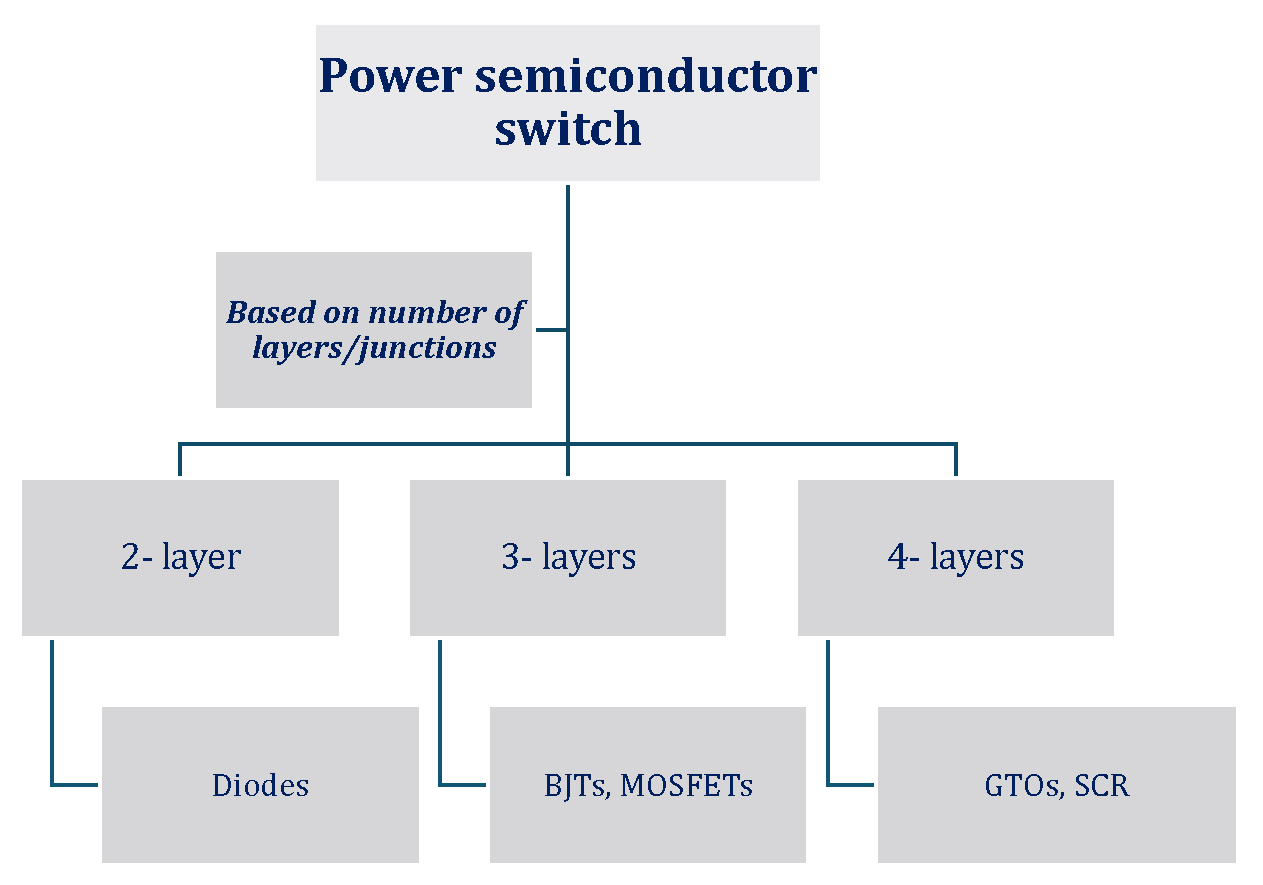
\includegraphics[scale=0.35]{fig/lec04/classification_of_device_2.eps}
            \caption{Classification of power semiconductor devices based on number of layers.}
        \end{figure}
    \end{columns}
\end{frame}

\begin{frame}
	\frametitle{Classification of types of power semiconductor devices}
    \textbf{Based on controllability:}
    \begin{columns}
        \column{0.35\textwidth}
        \begin{itemize}
            \item \textbf{Uncontrolled:}
            \begin{itemize}
                \item Diodes (e.g., Schottky, Zener, and standard rectifier diodes).
            \end{itemize}
            \item \textbf{Semicontrolled:}
            \begin{itemize}
                \item SCRs.
            \end{itemize}
            \item \textbf{Fully controlled:}
            \begin{itemize}
                \item BJTs.
                \item MOSFETs.
            \end{itemize}
        \end{itemize}

        \column{0.65\textwidth}
        \begin{figure}
            \centering
            \label{fig:Classification_based_on_controllability}
            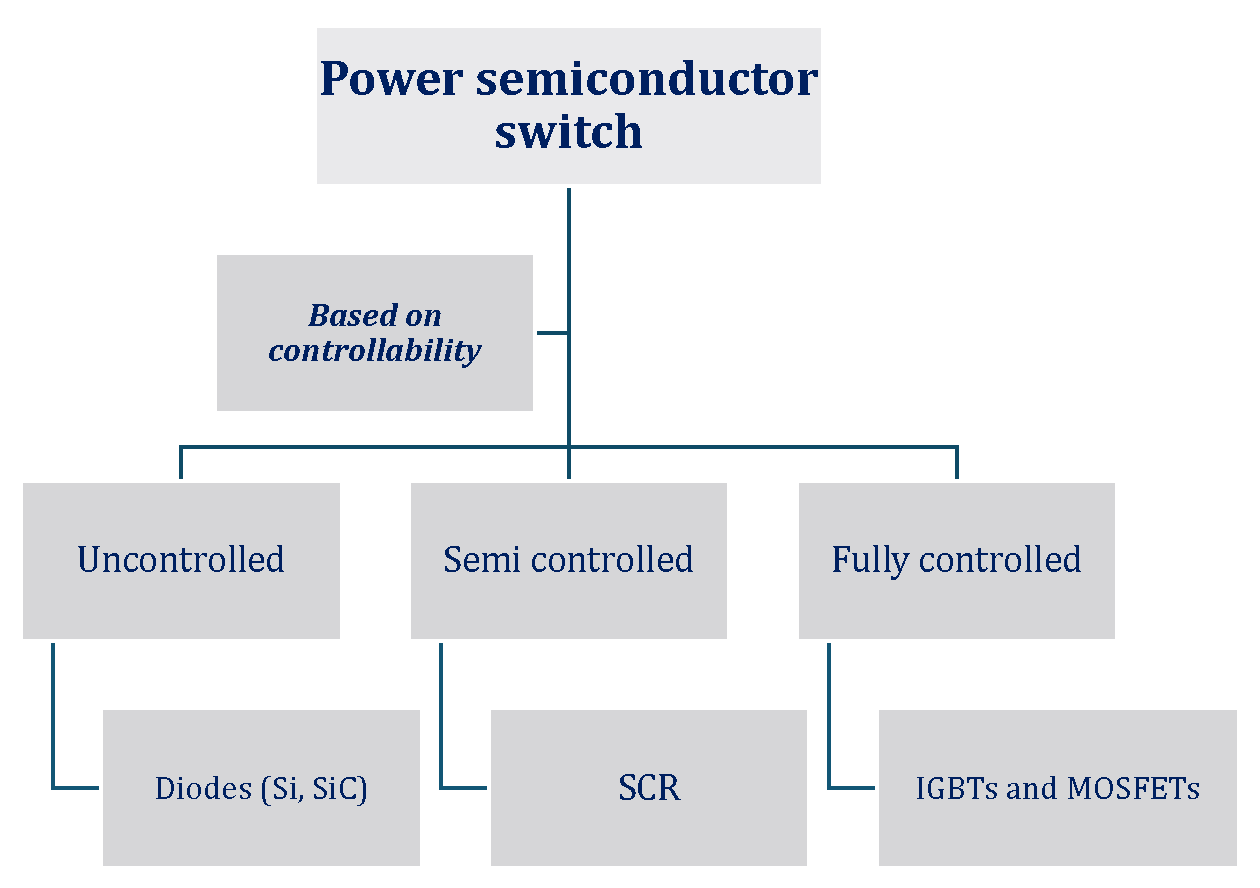
\includegraphics[scale=0.35]{fig/lec04/classification_of_device_3.eps}
            \caption{Classification of power semiconductor devices based on controllability.}
        \end{figure}
    \end{columns}
\end{frame}


\begin{frame}
	\frametitle{Classification of types of power semiconductor devices}
    \textbf{Based on quadrant of operation:}
    \begin{columns}
        \column{0.35\textwidth}
        \begin{itemize}
            \item \textbf{Single quadrant:}
            \begin{itemize}
                \item Diodes (e.g., Schottky, Zener, and standard rectifier diodes).
            \end{itemize}
            \item \textbf{Two quadrant:}
            \begin{itemize}
                \item Current bidirectional devices (e.g., MOSFETs).
                \item Voltage bidirectional devices (e.g., MOSFET with a series diodes).
            \end{itemize}
            \item \textbf{Four quadrant:}
            \begin{itemize}
                \item By combination of two or more devices (e.g., using IGBTs and MOSFETs).
                \item MOSFETs.
            \end{itemize}
        \end{itemize}

        \column{0.65\textwidth}
        \begin{figure}
            \centering
            \label{fig:Classification_based_on_quadrant_of_operation}
            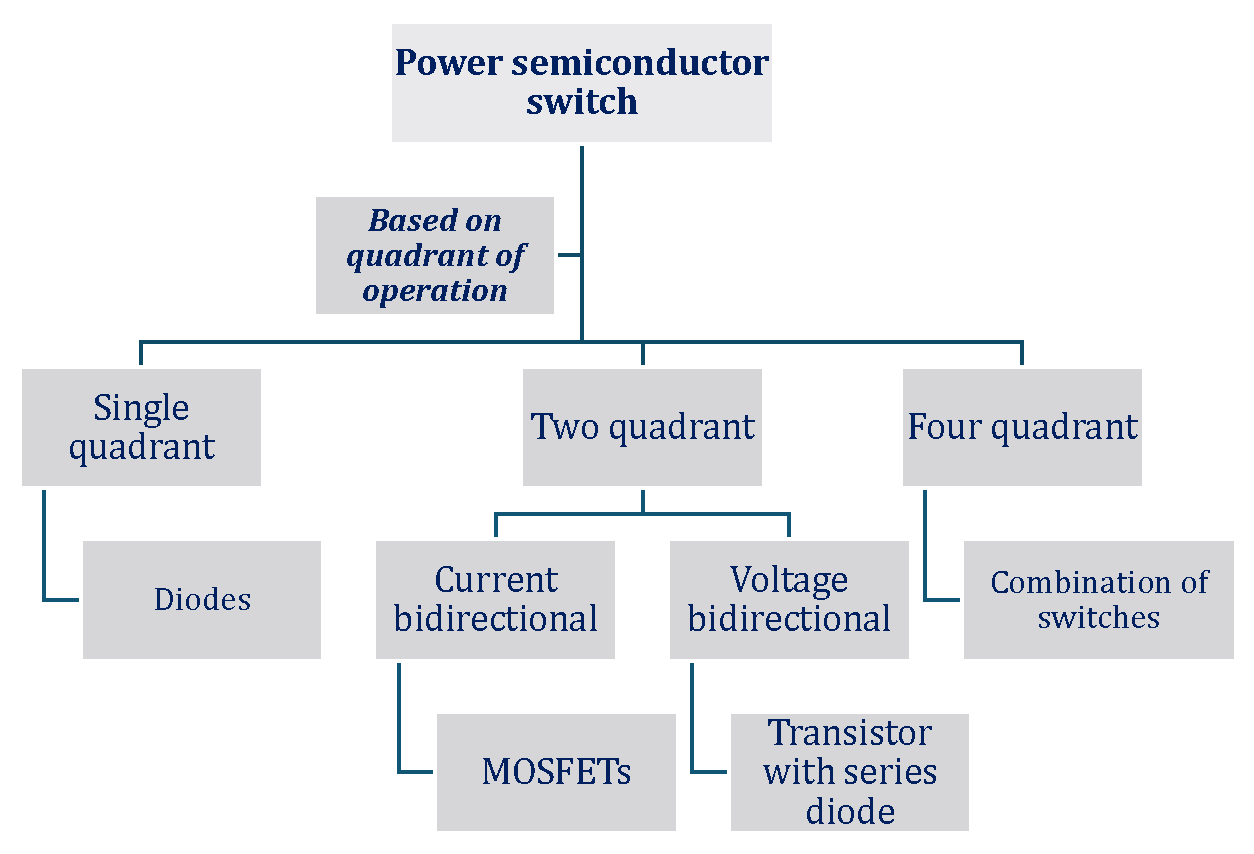
\includegraphics[scale=0.35]{fig/lec04/classification_of_device_4.eps}
            \caption{Classification of power semiconductor devices based on quadrant of operation.}
        \end{figure}
    \end{columns}
\end{frame}

%%%%%%%%%%%%%%%%%%%%%%%%%%%%%%%%%%%%%%%%%%%%%%%%%%%%%%%%%%%%%%%
%% Power Diodes %%
%%%%%%%%%%%%%%%%%%%%%%%%%%%%%%%%%%%%%%%%%%%%%%%%%%%%%%%%%%%%%%%
\begin{frame}
    \frametitle{Power Diodes}
    \textbf{1. Definition:} \\
    \textit{A power diode is a semiconductor device that allows current to flow in one direction while blocking it in the opposite direction. It is designed to handle high voltages and currents, making it suitable for power applications.}

    \textbf{2. Key Characteristics:}
    \begin{itemize}
        \item \textbf{Forward Voltage Drop (\(V_f\)):} The voltage drop across the diode when it is conducting.
        \item \textbf{Reverse Breakdown Voltage (\(V_{BR}\)):} The maximum reverse voltage the diode can withstand before breakdown occurs.
        \item \textbf{Reverse Recovery Time (\(t_{rr}\)):} The time taken for the diode to switch from conducting to blocking state.
    \end{itemize}

    \textbf{3. Types of Power Diodes:}
    \begin{itemize}
        \item \textbf{Standard Rectifier Diodes:} Used in AC-DC conversion.
        \item \textbf{Schottky Diodes:} Low forward voltage drop and fast switching; used in high-frequency applications.
        \item \textbf{Zener Diodes:} Used for voltage regulation and protection against overvoltage conditions.
    \end{itemize}
\end{frame}

\begin{frame}
    \frametitle{Power Diodes- basic structure}
    \begin{columns}
        \column{0.4\textwidth}
        \begin{itemize}
            \item \textbf{Basic Structure:}
            \begin{itemize}
                \item Inclusion of a lightly doped $n^-$ drift region.
                \begin{itemize}
                    \item the lightly doped $n^-$ layer (drift region) allows the depletion region to expand widely under reverse bias.
                    \item Allows the diode to have high voltage blocking capability
                \end{itemize}
                \item Thick epitaxial layer and high current capacity.
                \begin{itemize}
                    \item Epitaxial growth and cross-sectional area are tailored to high current rating.
                    \item Larger devices use 4-inch wafers.
                \end{itemize}
            \end{itemize}
        \end{itemize}

        \column{0.6\textwidth}
        \begin{figure}
            \centering
            \label{fig:Power_Diodes_structure_and_IV_characteristics}
            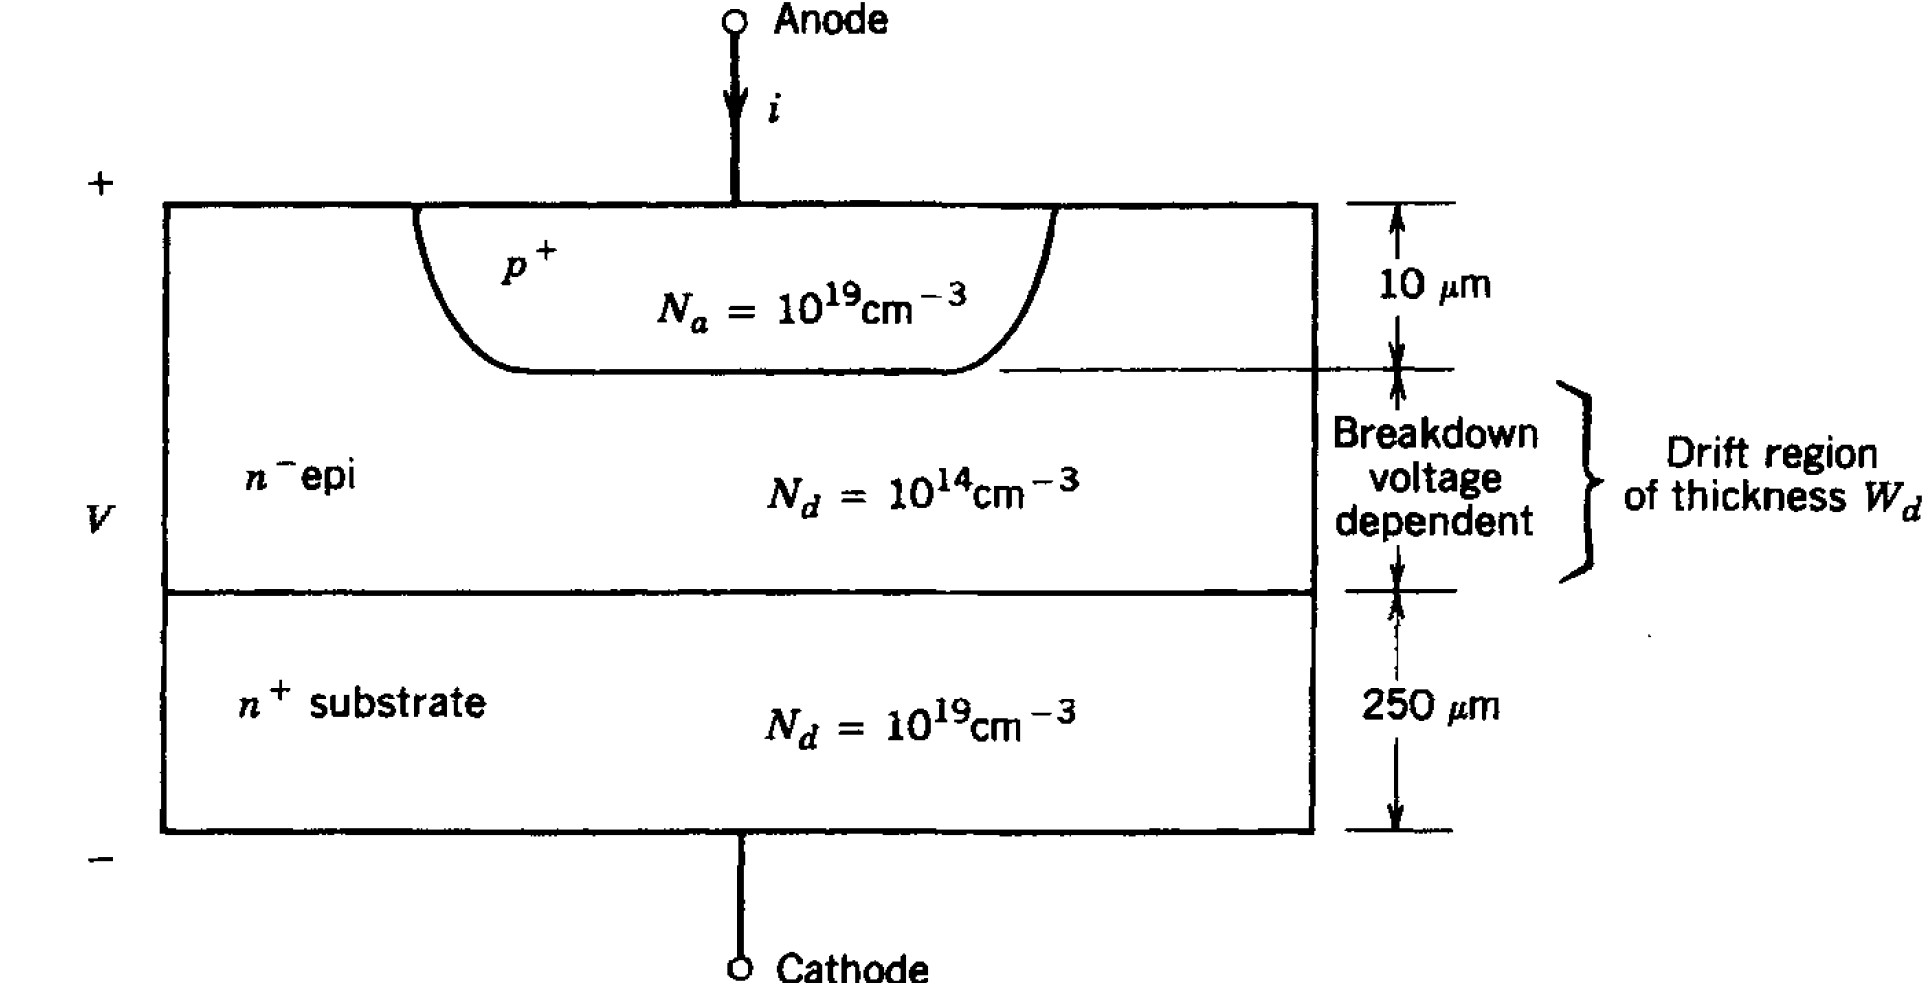
\includegraphics[scale=0.2]{fig/lec04/cross_section_pn_junction.png}
            \caption{Cross section of pn junction diode; adapted from Mohan, Undeland, Robbins, "Power Electronics: Converters, Applications and Design - 2nd Edition".}
        \end{figure}
    \end{columns}
\end{frame}

\begin{frame}
    \frametitle{Power Diodes- Static characteristics}
    \begin{columns}
        \column{0.45\textwidth}
        \begin{itemize}
            \item \textbf{Linear forward conduction:}
            \begin{itemize}
                \item high forward current flows through the lightly doped drift region, introducing significant series resistance $R_{on}$.
                \item The characteristic is linear rather than exponential beyond $\approx$ 1V.
            \end{itemize}
            \item \textbf{Reverse bias and avalanche breakdown:}
            \begin{itemize}
                \item Under reverse bias, a small leakage current flows until the breakdown voltage $BV_{BD}$ is reached.
                \item Beyond $BV_{BD}$ avalanche multiplication causes current to rise rapidly while the voltage remains approximately constant.
            \end{itemize}
            \item \textbf{Breakdown operation must be avoided!.}
        \end{itemize}

        \column{0.55\textwidth}
        \begin{figure}
            \centering
            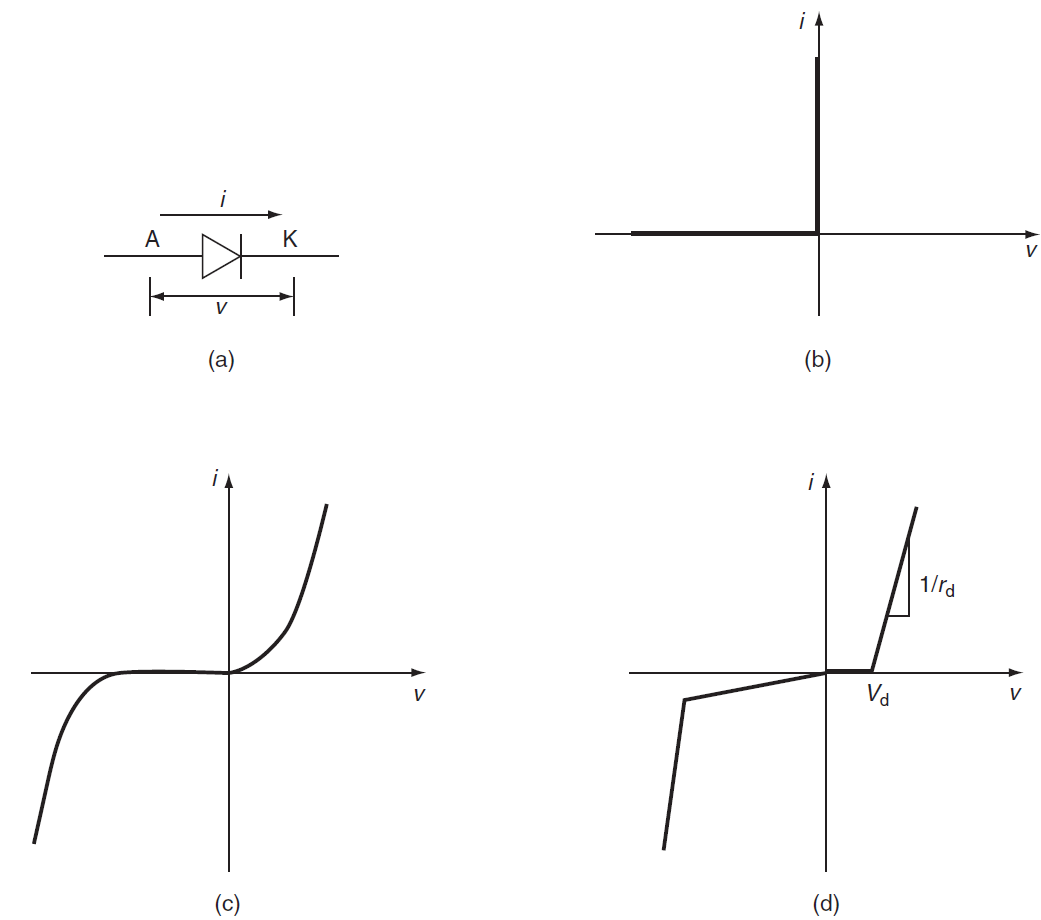
\includegraphics[scale=0.275]{fig/lec04/static_characteristics_diode.png}
            \caption{(a) symbol of diode, (b) ideal VI characteristics, (c) VI characteristics of a practical diode (d) piece wise linear model; adapted from Umanand, L., Power Electronics: Essentials \& Applications.}
            \label{fig:static_diode_characteristics}
        \end{figure}
    \end{columns}
\end{frame}

\begin{frame}
    \frametitle{Power Diodes- Dynamic characteristics}
    \begin{columns}
        \column{0.45\textwidth}
        \textbf{Turn-OFF of Diode:}
        \begin{itemize}
            \item When a forward-biased diode is suddenly reverse biased, excess carriers in the diffusion region (space-charge region) must be removed.
            \item The diode voltage remains in the ON-state initially due to stored charge.
            \item Reverse current flows until charges are removed at time $t_2$, after which the junction becomes reverse biased.
            \item The time interval from $t_1$ to $t_2$ is termed \textbf{storage time}, and $t_{rr}$ (total duration of reverse recovery) is crucial for switching applications.
        \end{itemize}
        \column{0.55\textwidth}
        \begin{figure}
            \centering
            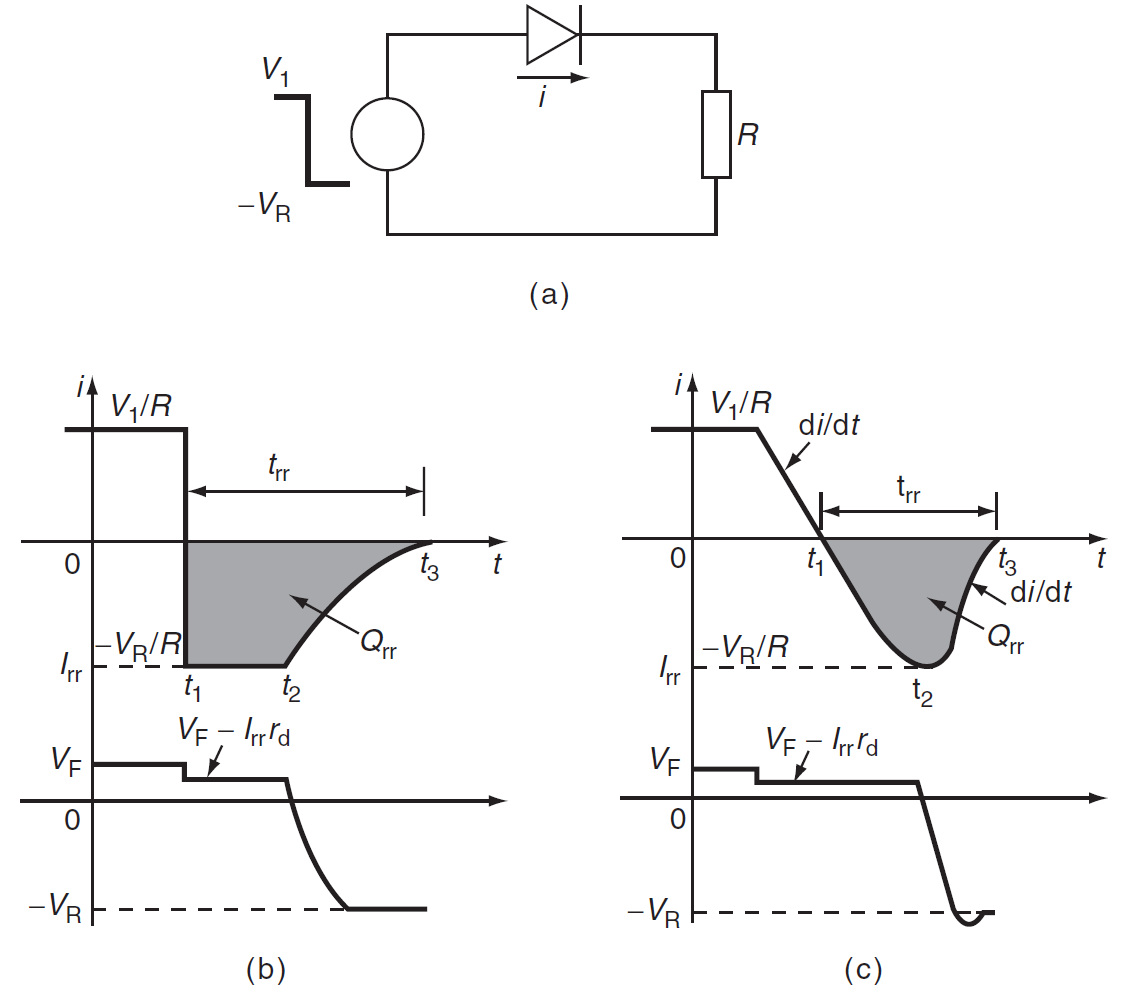
\includegraphics[scale=0.25]{fig/lec04/dynamic_characteristics_diode.png}
            \caption{(a) test circuit- turn-off, (b) ideal dynamic characteristics, (c) practical diode dynamic characteristics-turn-off; adapted from Umanand, L., Power Electronics: Essentials \& Applications.}
            \label{fig:dynamic_diode_characteristics}
        \end{figure}
    \end{columns}
\end{frame}

\begin{frame}
    \frametitle{Power Diodes- Dynamic characteristics}
    \begin{columns}
        \column{0.45\textwidth}
        \textbf{Turn-ON of Diode:}
        \begin{itemize}
            \item If a diode under reverse bias is forward biased, the transition requires a time known as \textbf{turn-ON time} or \textbf{forward recovery time}.
            \item Charges redistribute from to establish steady-state conduction.
            \item This process is generally faster than charge removal during turn-OFF, hence $t_{ON} < t_{OFF}$.
        \end{itemize}
        \vspace{0.2cm}
        \textit{Note: In practical circuits, reverse recovery can be slowed by parasitic inductance.}

        \column{0.55\textwidth}
        \begin{figure}
            \centering
            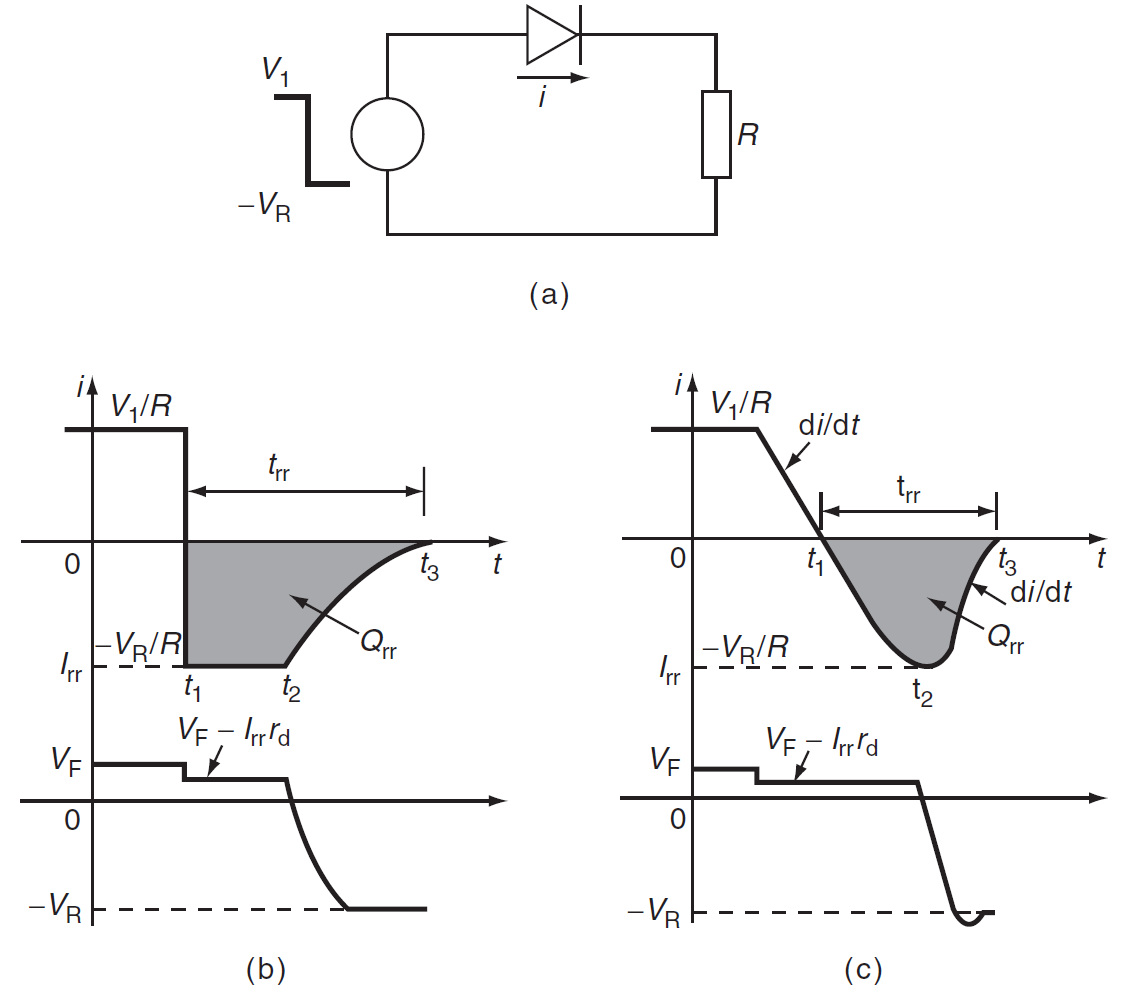
\includegraphics[scale=0.25]{fig/lec04/dynamic_characteristics_diode.png}
            \caption{(a) test circuit- turn-off, (b) ideal dynamic characteristics, (c) practical diode dynamic characteristics-turn-off; adapted from Umanand, L., Power Electronics: Essentials \& Applications.}
            \label{fig:dynamic_diode_characteristics}
        \end{figure}
    \end{columns}
\end{frame}

\begin{frame}{\textbf{Classification and Parameters of Power Diodes}}

    \textbf{Diode Classifications}
    \begin{itemize}
        \item Classification is based on reverse recovery time $t_{rr}$, indicating how quickly a diode can switch off.
        \item \textbf{Types of Diodes:}
        \begin{enumerate}
            \item \textbf{Rectifier Diodes:} $t_{rr}$ in the microsecond range.
            \item \textbf{Fast Recovery Diodes:} $t_{rr}$ between 200--500 ns.
            \item \textbf{Ultra-Fast Recovery Diodes:} $t_{rr} \sim$ 30--200 ns.
            \item \textbf{Schottky Diodes:} Metal-semiconductor junction, $t_{rr} <$ 30 ns.
        \end{enumerate}
        \item For high-frequency applications (e.g. SMPS, converters), use types 2--4 based on frequency and voltage ratings.
    \end{itemize}
    
    \textbf{Applications:}
    \begin{itemize}
        \item Type 1 is suitable for low-frequency mains rectification.
        \item Types 2--4 used in fast-switching converters.
    \end{itemize}
    
    \end{frame}
    
    \begin{frame}{\textbf{Datasheet Parameters for Diode Selection}}
    
    \textbf{Key Diode Parameters:}
    \begin{enumerate}
        \item Average forward current, $I_{\text{Fav}}$
        \item RMS forward current, $I_{\text{Frms}}$
        \item Peak forward current, $I_{\text{F}}$
        \item Surge current, $I_{\text{FSM}}$
        \item Breakdown or reverse voltage, $V_{\text{RRM}}$
        \item Forward voltage drop, $V_{\text{F}}$
        \item Dynamic resistance, $r_d$
        \item Reverse recovery time, $t_{rr}$
        \item Thermal endurance: $I^2t$ rating
    \end{enumerate}
    
    \textbf{Important Notes:}
    \begin{itemize}
        \item For sinusoidal operation, $I_{\text{Fav}}, I_{\text{Frms}}, I_{\text{F}}$ relations are well-known.
        \item For non-sinusoidal waveforms, these values must be derived from fundamentals.
        \item Choose diode ratings higher than the worst-case circuit values.
    \end{itemize}
    
    \end{frame}
    
    \begin{frame}{\textbf{Surge Current}}
        \textbf{Surge Current:}
        \begin{itemize}
            \item Diodes can handle overload currents briefly without damage.
            \item Key datasheet specs: $I_{\text{FSM}}$ (max peak half-cycle non-repetitive current) and $I^2t$ (energy dissipation).
            \item Surge current often arises when rectifier filters switch on with high peak voltages.
            \item Limiting devices (e.g., series resistors or fuses) ensure surge stays below $I^2t$ limit.
        \end{itemize}
    \end{frame}
        
\begin{frame}{\textbf{Thermal Viewpoint of Diodes}}
    \textbf{Thermal Viewpoint:}
    \begin{itemize}
        \item Total power loss: $P_d = P_{\text{on}} + P_{\text{off}} + P_{\text{switching}}$
        \item \textbf{On-state loss:}
        \begin{equation}
            P_{\text{on}} = \frac{1}{T} \int_0^T v(t)i(t)\, dt \approx (V_d \times I_{\text{avg}}) + (I_{\text{rms}}^2 \times r_d)
        \end{equation}
        \item \textbf{Switching loss:}
        \begin{equation}
            P_{\text{switching}} = E_{\text{switching}} \cdot f_s = \left( \frac{1}{2} Q_{\text{rr}} V_R \right) f_s
        \end{equation}
        \item Reverse recovery charge:
        \begin{equation}
            Q_{\text{rr}} = \frac{1}{2} t_{\text{rr}} I_{\text{rr}} \Rightarrow P_{\text{switching}} = \frac{1}{4} I_{\text{rr}} V_R t_{\text{rr}} f_s
        \end{equation}
        \item Junction temperature must remain below datasheet limit (e.g., 150$^\circ$C).
    \end{itemize}
\end{frame}


\begin{frame}{\textbf{Modeling a Power Diode: Steady-State and Transient Behavior}}
    \begin{columns}
        \begin{column}{0.48\textwidth}
            \textbf{Objective:} To model both static and dynamic characteristics of a diode for simulation and design purposes.
            \vspace{0.5em}
            \begin{itemize}
                \item \textbf{Steady-State Behavior:}
                \begin{itemize}
                    \item Current-voltage $(i_d$–$V_d)$ relationship is exponential:
                    \[
                        i_d = I_0\left(e^{\frac{V_d}{nV_T}} - 1\right)
                    \]
                    \item $R_s$: Series resistance due to bulk and contact resistance (non-zero in practice).
                \end{itemize}
            \end{itemize}
        \end{column}
        
        \begin{column}{0.48\textwidth}
            \begin{figure}
                \centering
                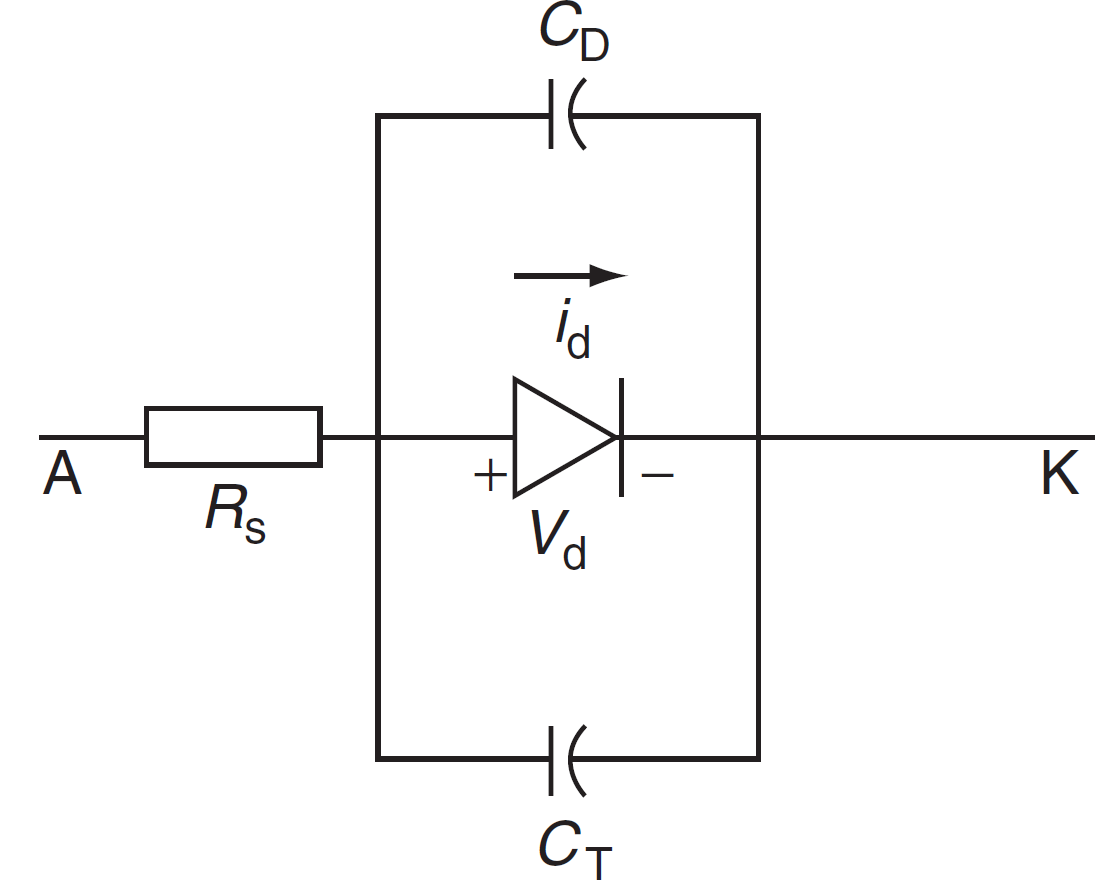
\includegraphics[scale=0.25]{fig/lec04/diode_model.png}
                \caption{Model of diode; adapted from Umanand, L., Power Electronics: Essentials \& Applications.}
                \label{fig:diode_model}
            \end{figure}
        \end{column}
    \end{columns}
    \end{frame}
    

\begin{frame}{\textbf{Modeling a Power Diode: Steady-State and Transient Behavior}}
    \begin{columns}
        \begin{column}{0.48\textwidth}
\begin{itemize}
\item \textbf{Dynamic Behavior:}
\begin{itemize}
    \item \textbf{Diffusion Capacitance ($C_D$):} 
        \begin{itemize}
            \item Appears during transition from forward to reverse bias.
            \item Models the excess mobile charge that must be removed.
        \end{itemize}
        
    \item \textbf{Transition Capacitance ($C_T$):}
        \begin{itemize}
            \item Relevant when transitioning from reverse to forward bias.
            \item Models mobile charge accumulation at the junction.
        \end{itemize}
\end{itemize}

\item \textbf{Capacitance Non-Linearity:}
    \begin{itemize}
        \item Both $C_D$ and $C_T$ are non-linear and depend on the charge distribution.
        \item Circuit simulators implement these models dynamically.
    \end{itemize}
\end{itemize}
\end{column}

\begin{column}{0.48\textwidth}
    \begin{figure}
        \centering
        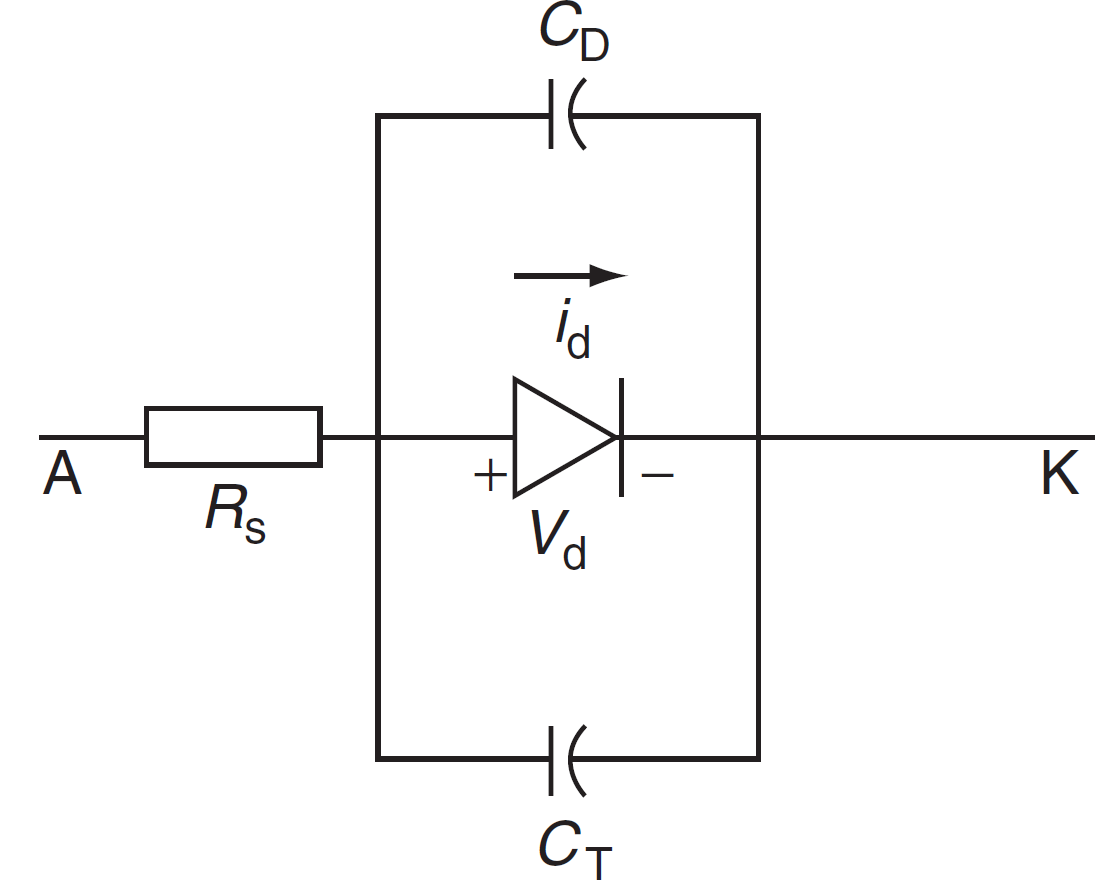
\includegraphics[scale=0.25]{fig/lec04/diode_model.png}
        \caption{Model of diode; adapted from Umanand, L., Power Electronics: Essentials \& Applications.}
        \label{fig:diode_model}
    \end{figure}
\end{column}
\end{columns}
\end{frame}

\begin{frame}{\textbf{Introduction to punch-through vs non-punch-through power diodes}}
    \textbf{Differences:Punch through vs non-punch-through:} 
    \centering
    \small
    \begin{tabular}{|p{3.5cm}|p{4cm}|p{4cm}|}
    \hline
    \textbf{Characteristic} & \textbf{Punch-through (PT)} & \textbf{Non-punch-through (NPT)} \\
    \hline
    Drift Region & Thinner, moderately doped & Thicker, lightly doped \\
    \hline
    Electric Field Profile & Extends through drift region (reaches anode) & Ends before reaching the anode \\
    \hline
    Breakdown Mechanism & Abrupt avalanche breakdown & Gradual breakdown onset \\
    \hline
    Switching Speed & Faster reverse recovery & Slower but more robust \\
    \hline
    On-State Voltage Drop & Lower & Slightly higher \\
    \hline
    Reverse Recovery Loss & Lower & Higher \\
    \hline
    Application Voltage Range & Medium (e.g., 600–1200 V) & High (e.g., >1200 V) \\
    \hline
    Example Devices & Transient Voltage Suppression and Schottky barrier diodes & 1N400x  \\
    \hline
    \end{tabular} \\
    \vspace{0.3cm}
    \textbf{Design Implication:} Choice depends on switching frequency, voltage class, and thermal constraints.
\end{frame}

\begin{frame}{\textbf{Avalanche Breakdown in Step Junctions}}
    \textbf{Concept:} Reverse bias in a $p$–$n$ junction causes the electric field to drop entirely across the depletion region. As the field strength increases, it approaches a critical value $E_{\text{BD}}$ where impact ionization begins $\Rightarrow$ Avalanche Breakdown.
    
    \vspace{0.3em}
    \textbf{Key Definitions:}
    \begin{itemize}
        \item \textbf{Breakdown Voltage} ($BV_{\text{BD}}$): Reverse-bias voltage at which impact ionization becomes significant.
        \item \textbf{Critical Field Strength} ($E_{\text{BD}}$): Electric field at which avalanche multiplication starts.
    \end{itemize}
    
    \vspace{0.3em}
    \textbf{Breakdown Condition:}
    \begin{equation}
        E_{\max} \approx E_{\text{BD}}
    \end{equation}
    \textbf{Where:}
    \begin{itemize}
        \item $E_{\max}$: Maximum electric field in the depletion region.
    \end{itemize}
\end{frame}
    
\begin{frame}{\textbf{Breakdown Voltage Expression for Step Junction}}
    \begin{equation}
    BV_{\text{BD}} = \phi_c + \left[ \frac{W_0 E_{\text{BD}}}{2 \varepsilon} \right]^2 - \phi_c \approx \frac{\varepsilon (N_A + N_D) E_{\text{BD}}^2}{2 q N_A N_D}
    \end{equation}
    
    \textbf{Parameters:}
    \begin{itemize}
        \item $W_0$: Depletion width
        \item $E_{\text{BD}}$: Breakdown electric field
        \item $\varepsilon$: Permittivity of the semiconductor
        \item $N_A, N_D$: Acceptor and donor concentrations
        \item $q$: Electron charge
        \item $\phi_c$: Contact potential
    \end{itemize}
    
    \vspace{0.3em}
    \textbf{Observation:} Breakdown voltage depends strongly on doping concentrations and junction profile (e.g., step, graded, diffused).
\end{frame}


\begin{frame}{\textbf{Breakdown Voltage in Non-Punch-Through (NPT) Diodes}}

    \textbf{Structure Concept:}
    \begin{itemize}
        \item \textbf{Non-punch-through diode:} Drift region thickness $W_d$ is \textit{greater than} depletion width at breakdown.
        \item Depletion region does \textbf{not reach} the heavily doped $n^+$ substrate.
    \end{itemize}
    
    \vspace{0.4em}
    \textbf{Simplified Breakdown Voltage Equation:}
    \begin{equation}
        BV_{\text{BD}} \approx \frac{\varepsilon E_{\text{BD}}^2}{2 q N_D}
    \end{equation}
    \begin{itemize}
        \item $E_{\text{BD}}$: Breakdown electric field
        \item $N_D$: Doping concentration of drift region (lightly doped $n$)
        \item $\varepsilon$: Permittivity of the semiconductor
    \end{itemize}
    
\end{frame}

\begin{frame}{\textbf{Breakdown Voltage in Non-Punch-Through (NPT) Diodes}}

\textbf{Numerical Estimation for Silicon:}
\begin{equation}
    BV_{\text{BD}} \approx \frac{1.3 \times 10^{17}}{N_D}
\end{equation}
(for $N_D$ in $\text{cm}^{-3}$, $BV_{\text{BD}}$ in volts)

\vspace{0.4em}
\textbf{Depletion Width at Breakdown:}
\begin{equation}
    W_d \approx \frac{2 BV_{\text{BD}}}{E_{\text{BD}}} \approx 10^{-5} BV_{\text{BD}} \quad \text{(in cm)}
\end{equation}

\vspace{0.4em}
\textbf{Design Implications:}
\begin{itemize}
    \item High breakdown voltages $\Rightarrow$ require very \textbf{light doping} ($\sim 10^{14}$ cm$^{-3}$).
    \item Drift region width for 1000 V breakdown $\approx$ 100 $\mu$m.
    \item Trade-off between \textbf{blocking capability} and \textbf{on-resistance}.
\end{itemize}
\end{frame}

\begin{frame}{\textbf{Punch-Through Diode Breakdown Mechanism}}
    \begin{columns}
    
    \begin{column}{0.5\textwidth}
    \textbf{Definition:} Punch-through occurs when the reverse bias extends the depletion region entirely across the lightly doped $n^-$ drift region up to the heavily doped $n^+$ region.
    
    \begin{itemize}
        \item Reverse bias pushes the depletion edge to contact $n^+$, beyond which it cannot grow.
        \item The electric field profile changes shape — not triangular anymore.
        \item Breakdown voltage is reached when $E_1 + E_2 = E_{BD}$.
    \end{itemize}
    
    \vspace{1em}
    \textbf{Key Point:} The $n^+$ layer's heavy doping blocks further depletion region growth.
    \end{column}
    
    \begin{column}{0.5\textwidth}
    \begin{figure}
        \centering
        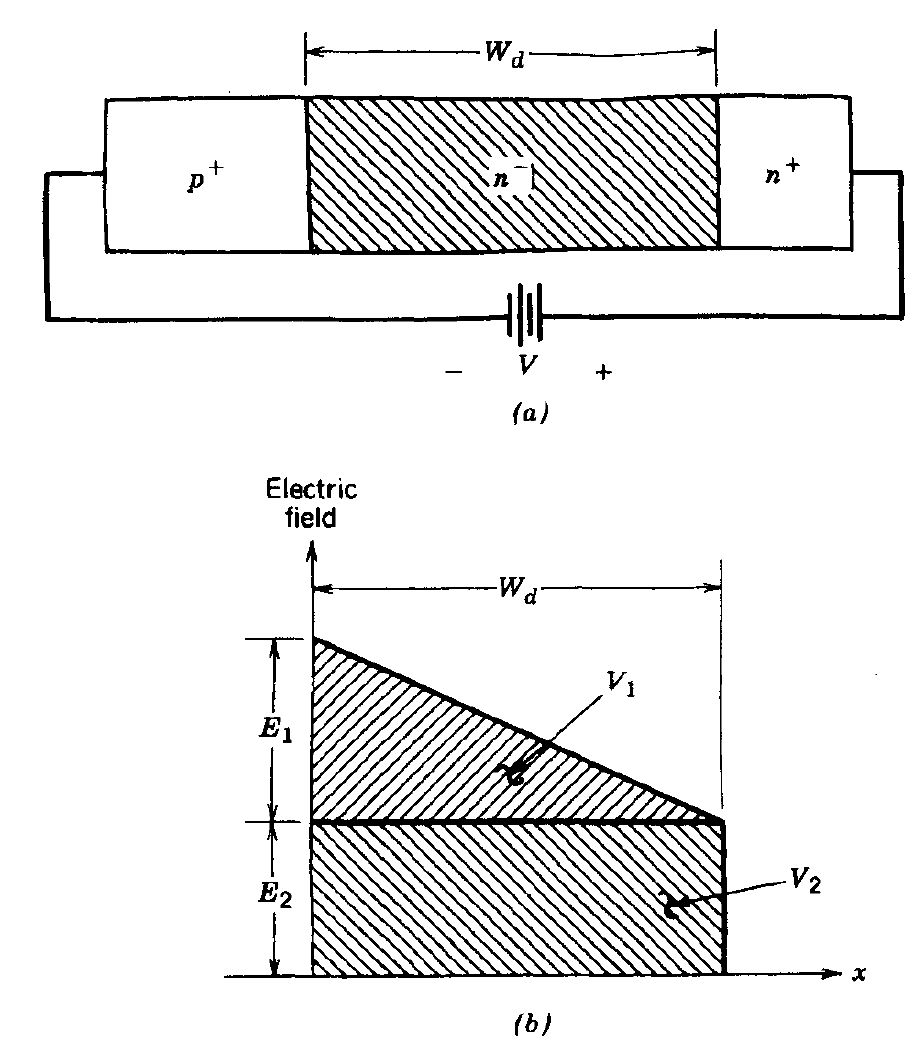
\includegraphics[scale=0.25]{fig/lec04/punch_through.png}
        \caption{\scriptsize Punch-through diode under reverse bias: (a) Depletion layer extends fully across the drift region (punch-through condition); (b) Electric field profile. Adapted from Mohan et al., \textit{Power Electronics, 2nd Ed.}}
        \label{fig:punch_through_diode}
    \end{figure}
    \end{column}
    
    \end{columns}
\end{frame}


\begin{frame}{\textbf{Electric Field \& Voltage Profile in Punch-Through Diode}}
    \begin{itemize}
        \item Electric field profile:
        \begin{itemize}
            \item Triangular portion: $E_1 = \frac{qN_dW_d}{\varepsilon}$
            \item Rectangular portion: $E_2$
        \end{itemize}
        \item Breakdown voltage:
        \begin{equation}
            V_1 = \frac{qN_dW_d^2}{2\varepsilon}, \quad V_2 = E_2 W_d
        \end{equation}
        \begin{equation}
            BV_{BD} = V_1 + V_2 = E_{BD}W_d - \frac{qN_dW_d^2}{2\varepsilon}
        \end{equation}
    \end{itemize}
    \textbf{Observation:} When $V_1 \ll V_2$, then $BV_{BD} \approx E_{BD}W_d$
\end{frame}

\begin{frame}{\textbf{Implications of Punch-Through Design}}
    \begin{itemize}
        \item Allows shorter $W_d$ for same $BV_{BD}$ → compact device.
        \item Higher resistivity in drift region increases $R_{on}$:
        \begin{itemize}
            \item Higher conduction loss compared to non-punch-through.
        \end{itemize}
        \item \textbf{Important:} No conductivity modulation under on-state — no conductivity injection from minority carriers.
        \item Results in higher $R_{on}$ under on-state condition.
    \end{itemize}
    \textbf{Conclusion:} Useful for high-speed, high-frequency operation despite higher on-resistance.
\end{frame}

\begin{frame}{\textbf{Schottky Diode: Structure and Principle of Operation}}
    \begin{columns}
        \begin{column}{0.6\textwidth}
        \textbf{Structure:}
        \begin{itemize}
            \item Formed by placing a metal in contact with an $n$-type semiconductor.
            \item The metal acts as the anode and the semiconductor as the cathode.
            \item Only majority carriers (electrons in $n$-type) participate — no hole injection.
        \end{itemize}
        
        \textbf{Principle of Operation:}
        \begin{itemize}
            \item Barrier formed due to work function difference.
            \item Equilibrium is reached when electron flow from metal to semiconductor balances opposite flow.
            \item No minority carriers $\Rightarrow$ no charge storage $\Rightarrow$ fast switching.
        \end{itemize}
    \end{column}
    \begin{column}{0.4\textwidth}
                \begin{figure}
                    \centering
                    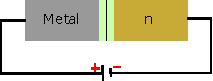
\includegraphics[scale=1]{fig/lec04/schottky_diode.pdf}
                    \caption{Schottky diode structure and energy band diagram; adapted from Mohan et al., \textit{Power Electronics, 2nd Ed.}}
                    \label{fig:schottky_diode_structure}
                \end{figure}
    \end{column}
\end{columns}
\end{frame}

\begin{frame}{\textbf{I-V Characteristics of Schottky Diode}}
    \begin{columns}
        \begin{column}{0.6\textwidth}
        \textbf{Equation:}
        \begin{equation}
        I = I_s \left( e^{\frac{qV}{nkT}} - 1 \right)
        \end{equation}
        
        \textbf{Key Observations:}
        \begin{itemize}
            \item Forward drop: 0.3–0.4 V (lower than silicon $p$-$n$ junction).
            \item High reverse leakage current due to majority-carrier injection.
            \item Not suitable beyond 100–200 V breakdown.
        \end{itemize}
        \textbf{Advantage:} Very fast ON/OFF response due to absence of stored charge.
    \end{column}
    \begin{column}{0.4\textwidth}
                \begin{figure}
                    \centering
                    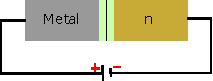
\includegraphics[scale=1]{fig/lec04/schottky_diode.pdf}
                    \caption{Schottky diode structure and energy band diagram; adapted from Mohan et al., \textit{Power Electronics, 2nd Ed.}}
                    \label{fig:schottky_diode_structure}
                \end{figure}
    \end{column}
\end{columns}

\end{frame}
    
\begin{frame}{\textbf{Ohmic vs Rectifying Contact in Metal–Semiconductor Junctions}}
    \textbf{Ohmic Contact:}
    \begin{itemize}
        \item No rectifying behavior; linear I-V characteristics.
        \item Occurs when metal work function $\phi_m < \phi_s$.
        \begin{itemize}
        \item The work function $\phi$ is the minimum energy needed to remove an electron from the Fermi level to vacuum.
        \item $\phi_m$ = work function of metal
        \item $\phi_s$ = work function (or electron affinity + energy gap position) of the semiconductor
    \end{itemize}
        \item Heavy doping or tunneling required to minimize barrier.
    \end{itemize}
    
    \textbf{Rectifying (Schottky) Contact:}
    \begin{itemize}
        \item Barrier prevents majority carriers $\Rightarrow$ diode action.
        \item No minority carrier injection $\Rightarrow$ low switching loss.
    \end{itemize}

\end{frame}

\begin{frame}{\textbf{Breakdown Behavior of Schottky Diodes}}
    \begin{itemize}
        \item Geometry and electric field crowding limits breakdown voltage.
        \item Surface effects and field curvature reduce breakdown to $\sim$200 V.
        \item No conductivity modulation $\Rightarrow$ higher drift region resistance.
        \item Trade-off: High $V_{BD}$ $\Rightarrow$ low doping $\Rightarrow$ high $R_{on}$.
    \end{itemize}
    \textbf{Comparison:} $p$-$n$ junction diodes can go to $\sim$5 kV due to conductivity modulation.
    \begin{itemize}
        \item Geometry and electric field crowding limits breakdown voltage.
        \item Surface effects and field curvature reduce breakdown to $\sim$200 V.
        \item No conductivity modulation $\Rightarrow$ higher drift region resistance.
        \item Trade-off: High $V_{BD}$ $\Rightarrow$ low doping $\Rightarrow$ high $R_{on}$.
    \end{itemize}
    \textbf{Comparison:} $p$-$n$ junction diodes can go to $\sim$5 kV due to conductivity modulation.
\end{frame}

\begin{frame}{\textbf{Switching Characteristics of Schottky Diodes}}
    \begin{itemize}
        \item Turn-ON and turn-OFF are extremely fast (no minority carrier storage).
        \item No reverse recovery current unlike $p$-$n$ diodes.
        \item Higher junction capacitance $\Rightarrow$ small voltage overshoot if $di/dt$ is large.
    \end{itemize}
    
    \textbf{Applications:} Preferred in high-frequency power converters and fast rectifiers. \\
    \textbf{Schottky Diode: Key Takeaways}
    \begin{itemize}
        \item Majority-carrier device with fast switching.
        \item Lower forward voltage drop (0.3–0.4 V).
        \item Poor high-voltage blocking ($<200$ V).
        \item Higher reverse leakage current than $p$-$n$ diodes.
        \item Ideal for low-voltage, high-speed power circuits.
    \end{itemize}
\end{frame}
    


\subsection{Power bipolar junction transistor (BJT)}

\begin{frame}
    \frametitle{Power bipolar junction transistor (BJT)}
    \textbf{1. Definition:} \\
    \textit{A power BJT is a three-terminal semiconductor device that can amplify or switch electronic signals and electrical power. It consists of two p-n junctions and is designed to handle high voltages and currents, making it suitable for power applications.}
\begin{itemize}
    \item Power BJTs require high blocking voltage in OFF state and high current capacity in ON state.
    \item Structure differs from logic-level BJTs to meet power handling demands.
    \item Exhibits distinct $i$–$v$ characteristics and switching behavior compared to signal BJTs.
    \item Applications include:
    \begin{itemize}
        \item Power converters
        \item Motor drives
        \item High-voltage switching circuits
    \end{itemize}
\end{itemize}
\end{frame}

\begin{frame}{\textbf{Bipolar Power Transistors (BJT)}}
\begin{itemize}
    \item BJTs are three-terminal current-controlled devices with:
    \begin{itemize}
        \item Emitter (E)
        \item Base (B)
        \item Collector (C)
    \end{itemize}
    \item Two types: \textbf{NPN} and \textbf{PNP}
    \item Current controlled: Small base current controls large collector current
    \item Can only conduct in one direction:
    \begin{itemize}
        \item NPN: C $\rightarrow$ E
        \item PNP: E $\rightarrow$ C
    \end{itemize}
    \item Structure: vertically oriented layers with heavily doped emitter and lightly doped collector
\end{itemize}
\begin{figure}
    \centering
    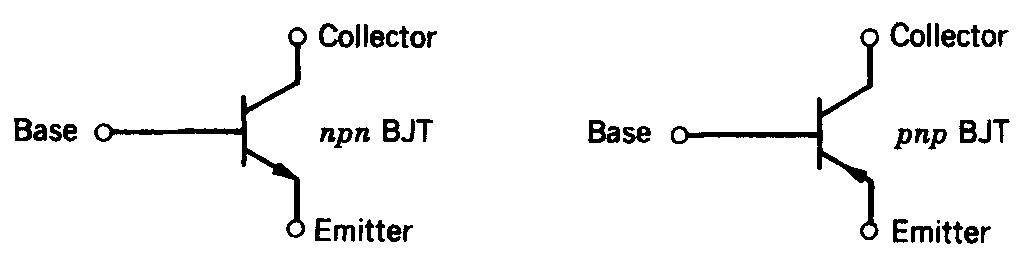
\includegraphics[width=0.5\linewidth]{fig/lec04/pnp_npn.png}
    \caption{BJT structure and symbol, adapted from Ned Mohan, Tore M. Undeland, and William P. Robbins, Power Electronics: Converters, Applications, and Design, 3rd Edition.}
    \label{fig:bjt_structure}
\end{figure}
\end{frame}

\begin{frame}{\textbf{Vertical Power Transistor Structure}}
    \begin{columns}
        \begin{column}{0.35\textwidth}
            \begin{itemize}
                \item 4-layer vertical structure with alternating $p$ and $n$-type regions.
                \item Base input, collector output, emitter common terminal.
                \item Vertical layout reduces $R_{\text{on}}$ and thermal resistance.
                \item Enhances current flow and reduces power dissipation.
                \item Common-emitter configuration used in power circuits.
            \end{itemize}
        \end{column}
    
        \begin{column}{0.65\textwidth}
            \begin{figure}
                \centering
                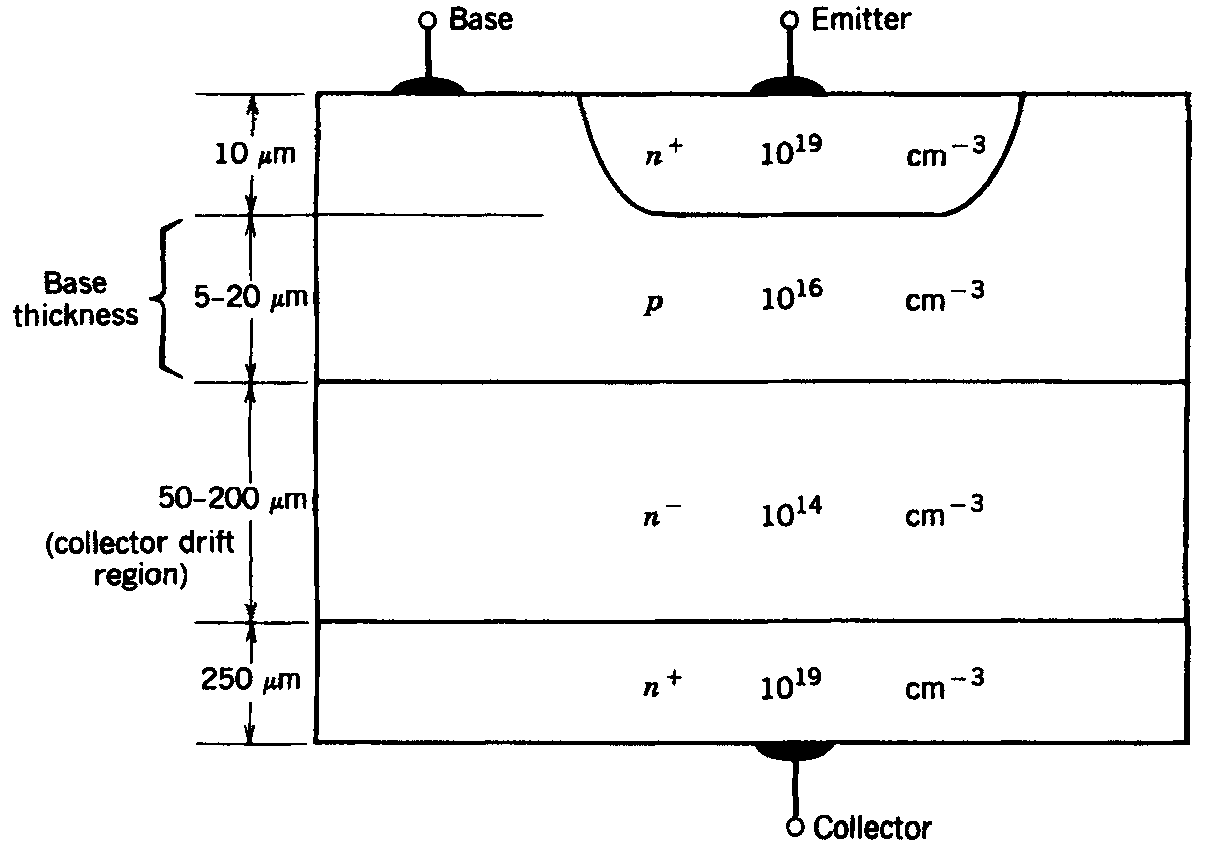
\includegraphics[scale=0.25]{fig/lec04/vertical_BJT_structure.png}
                \caption{Cross-section of a typical vertical $npn$ power BJT, adapted from Ned Mohan, Tore M. Undeland, and William P. Robbins, Power Electronics: Converters, Applications, and Design, 3rd Edition.}
            \end{figure}
        \end{column}
    \end{columns}
\end{frame}

\begin{frame}{\textbf{Doping and Thickness in Vertical BJTs}}
        \begin{columns}
        \begin{column}{0.35\textwidth}
            \begin{itemize}
                \item Emitter: Heavily doped $n^+$ ($\sim 10^{19}~\text{cm}^{-3}$)
                \item Base: Moderately doped $p$-type ($\sim 10^{16}~\text{cm}^{-3}$)
                \item Collector drift: Lightly doped $n^-$ ($\sim 10^{14}~\text{cm}^{-3}$), width = 50–200 $\mu$m
                \item Collector contact: $n^+$ ($\sim 10^{19}~\text{cm}^{-3}$)
            \end{itemize}
            \textbf{Design Considerations:}
            \begin{itemize}
                \item Base kept thin (5–20 $\mu$m) for high current gain.
                \item Drift region determines breakdown voltage.
            \end{itemize}
        \end{column}

        \begin{column}{0.65\textwidth}
            \begin{figure}
                \centering
                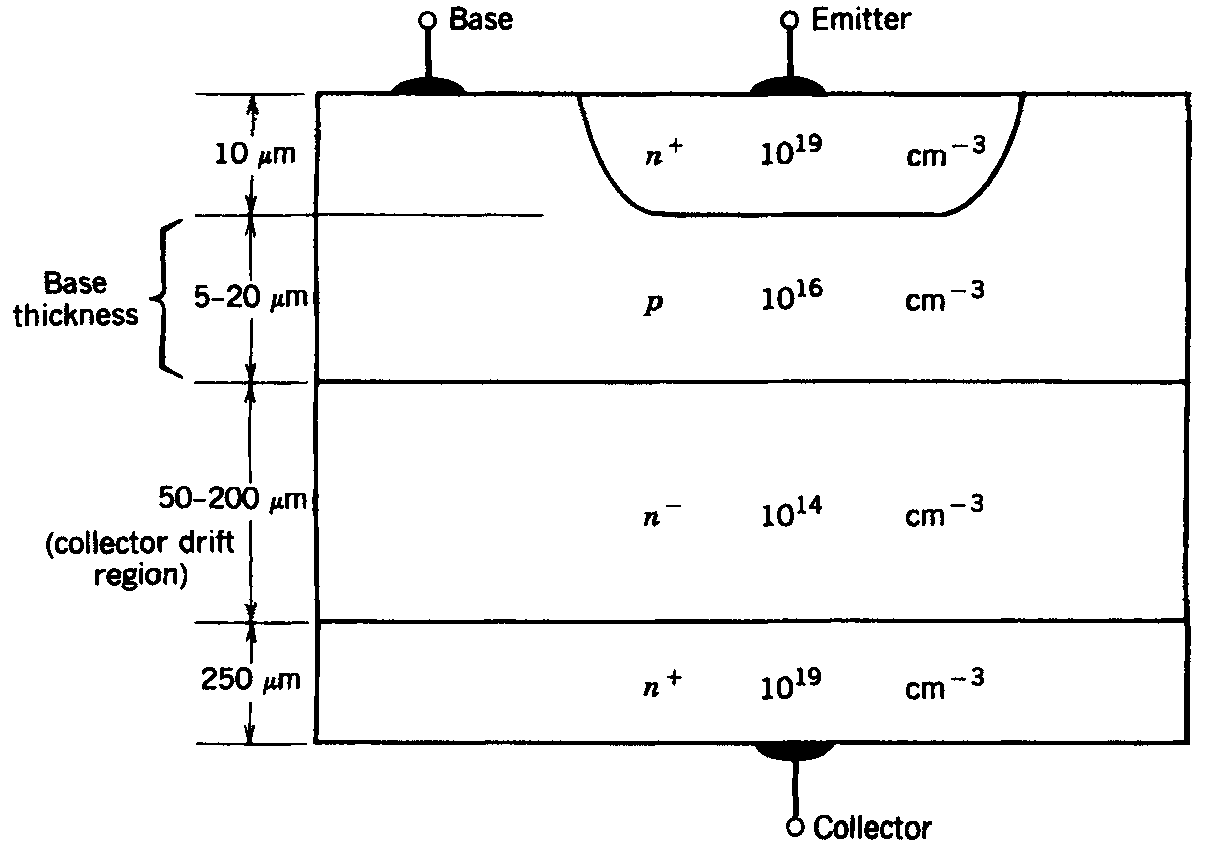
\includegraphics[scale=0.25]{fig/lec04/vertical_BJT_structure.png}
                \caption{Cross-section of a typical vertical $npn$ power BJT, adapted from Ned Mohan, Tore M. Undeland, and William P. Robbins, Power Electronics: Converters, Applications, and Design, 3rd Edition.}
            \end{figure}
        \end{column}
    \end{columns}
\end{frame}


\begin{frame}{\textbf{NPN Transistor: Operating Principle}}
    \begin{columns}
    \begin{column}{0.5\textwidth}
        \textbf{Operation:}
        \begin{itemize}
            \item Emitter–Base junction forward-biased $\rightarrow$ injects electrons into base.
            \item Base–Collector junction reverse-biased $\rightarrow$ collects electrons.
            \item Base is thin and lightly doped to minimize recombination.
            \item Electrons diffuse across base and are swept into collector.
            \item Base current $I_B$ is small; Collector current $I_C$ is large.
        \end{itemize}
        \textbf{Collector current:}
        \begin{equation}
            I_C = \alpha_F I_E - I_{CO}(e^{V_{CE}/V_T} - 1)
        \end{equation}
    \end{column}
    \begin{column}{0.5\textwidth}
        \begin{figure}
            \centering
            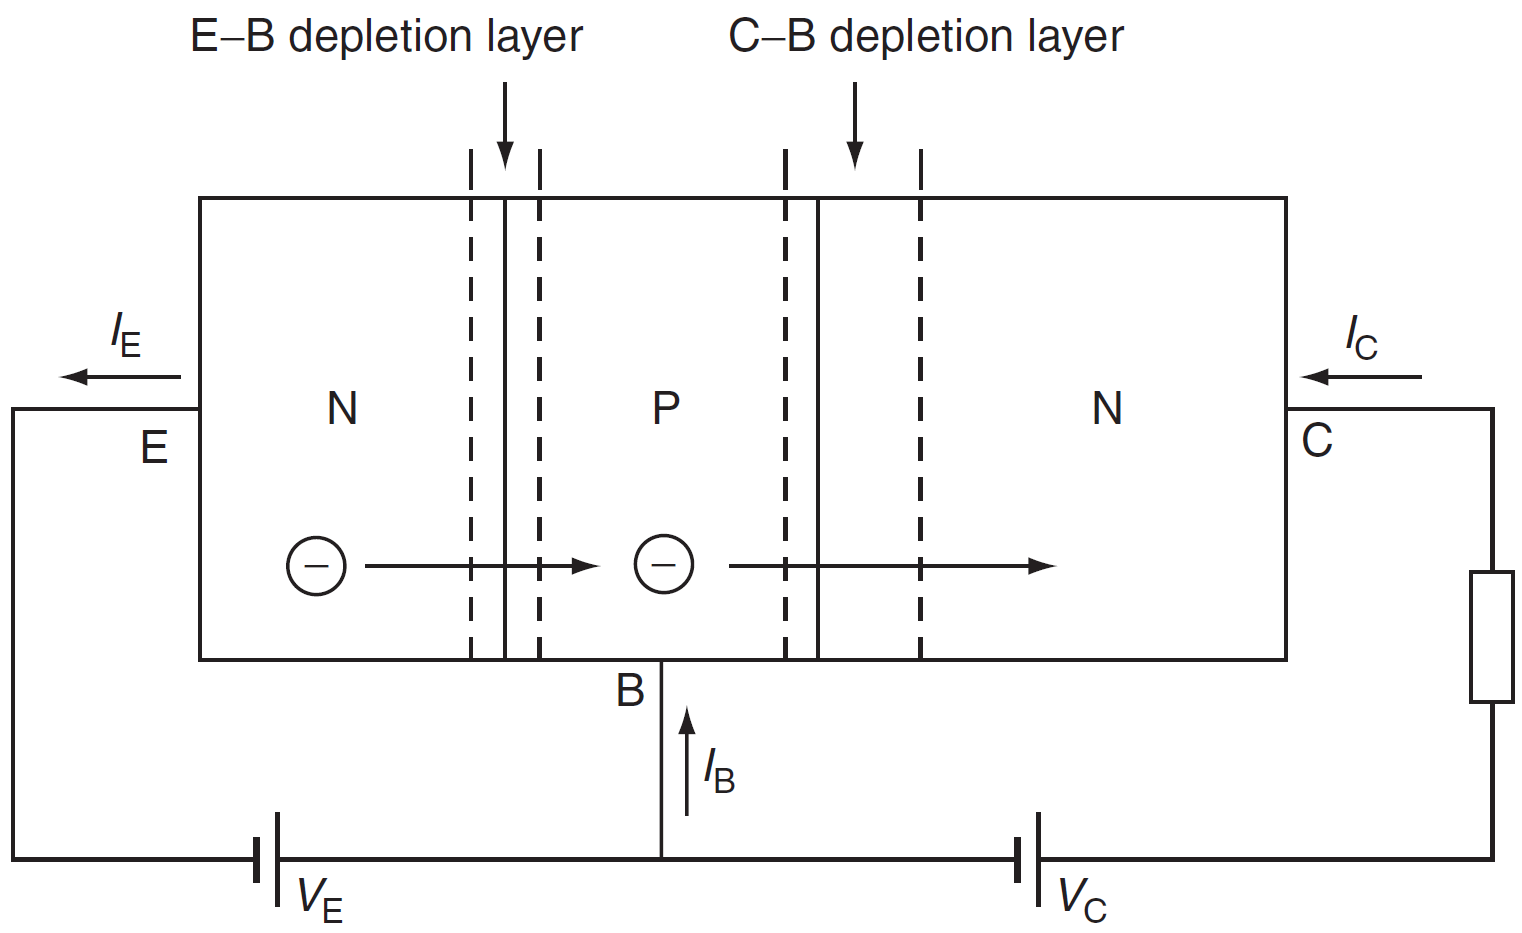
\includegraphics[width=0.8\linewidth]{fig/lec04/npn_bjt_operation.png}
            \caption{NPN BJT operation under forward active mode; adapted from Mohan et al., \textit{Power Electronics, 2nd Ed.}}
            \label{fig:npn_bjt_operation}
        \end{figure}
        \textbf{Emitter current:}
        \begin{equation}
        I_E = \alpha_R I_C - I_{EO}(e^{V_{EC}/V_T} - 1)
        \end{equation}
    \end{column}
  \end{columns}
\end{frame}

\begin{frame}{\textbf{BJT Current Components and Ebers-Moll Model}}
        \begin{columns}
    \begin{column}{0.4\textwidth}
        \begin{itemize}
            \item BJT modeled using Ebers-Moll equivalent circuit
            \item Includes forward and reverse $\alpha$ parameters
            \item Defines base, collector, and emitter currents via diode current equations
        \end{itemize}
        \begin{align*}
        I_C &= \alpha_F I_F - I_{CO}(e^{V_{CE}/V_T} - 1) \\
        I_E &= \alpha_R I_R - I_{EO}(e^{V_{EC}/V_T} - 1)
        \end{align*}
        \textbf{Current continuity:} $I_C + I_E + I_B = 0$
    \end{column}
    \begin{column}{0.6\textwidth}
        \begin{figure}
            \centering
            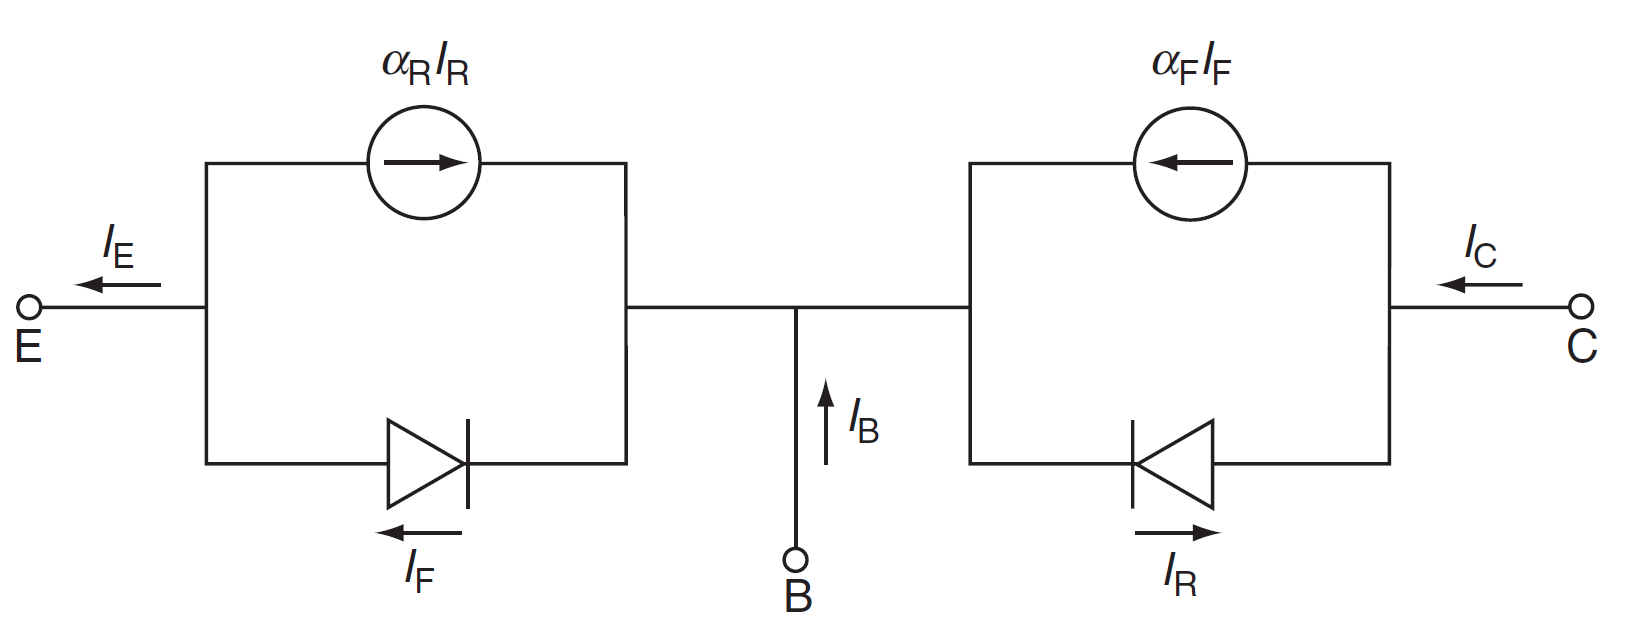
\includegraphics[width=0.8\linewidth]{fig/lec04/NPN_BJT_eq_model.png}
            \caption{Ebers-Moll equivalent circuit of NPN BJT}
        \end{figure}
    \end{column}
  \end{columns}
\end{frame}

\begin{frame}{\textbf{Key Parameters and Insights}}
\begin{itemize}
    \item $\alpha_F = \frac{I_C}{I_E}$ (forward common-base current gain), typically 0.9 to 0.98
    \item $\alpha_R = \frac{I_E}{I_R}$ (reverse common-base current gain), typically 0.02 to 0.1
    \item $\alpha_R$ is usually much smaller than $\alpha_F$.
    \item $\beta = \frac{I_C}{I_B}$ (common-emitter current gain), typically 50 to 200
    \item Higher $\alpha$ → better carrier injection from emitter
    \item Thin base → high efficiency but increased risk of punch-through
    \item $I_B$ is small but essential for switching control
\end{itemize}
\vspace{0.5em}
\textbf{Conclusion:} BJT operates via minority carrier injection and diffusion under strong forward bias conditions. It is highly efficient for amplification and switching when designed with proper base width and doping gradients.
\end{frame}


\begin{frame}{\textbf{BJT Current Gain Mechanism and Base Transport}}
\begin{columns}
\begin{column}{0.6\textwidth}
\textbf{Active Region Operation:}
\begin{itemize}
    \item In the active mode of a BJT, the base-emitter junction is forward biased, and the base-collector junction is reverse biased.
    \item Electrons are injected from the emitter (n$^+$) into the base (p) and then diffuse toward the collector.
    \item The base is intentionally kept very thin and lightly doped to minimize recombination and ensure most electrons reach the collector.
    \item The resulting collector current $I_C$ is almost equal to the emitter current $I_E$, while the base current $I_B$ remains small.
\end{itemize}

\textbf{Implication:} The small base current and large collector current results in current gain $\beta = \frac{I_C}{I_B}$.
\end{column}

\begin{column}{0.4\textwidth}
\begin{figure}
    \centering
    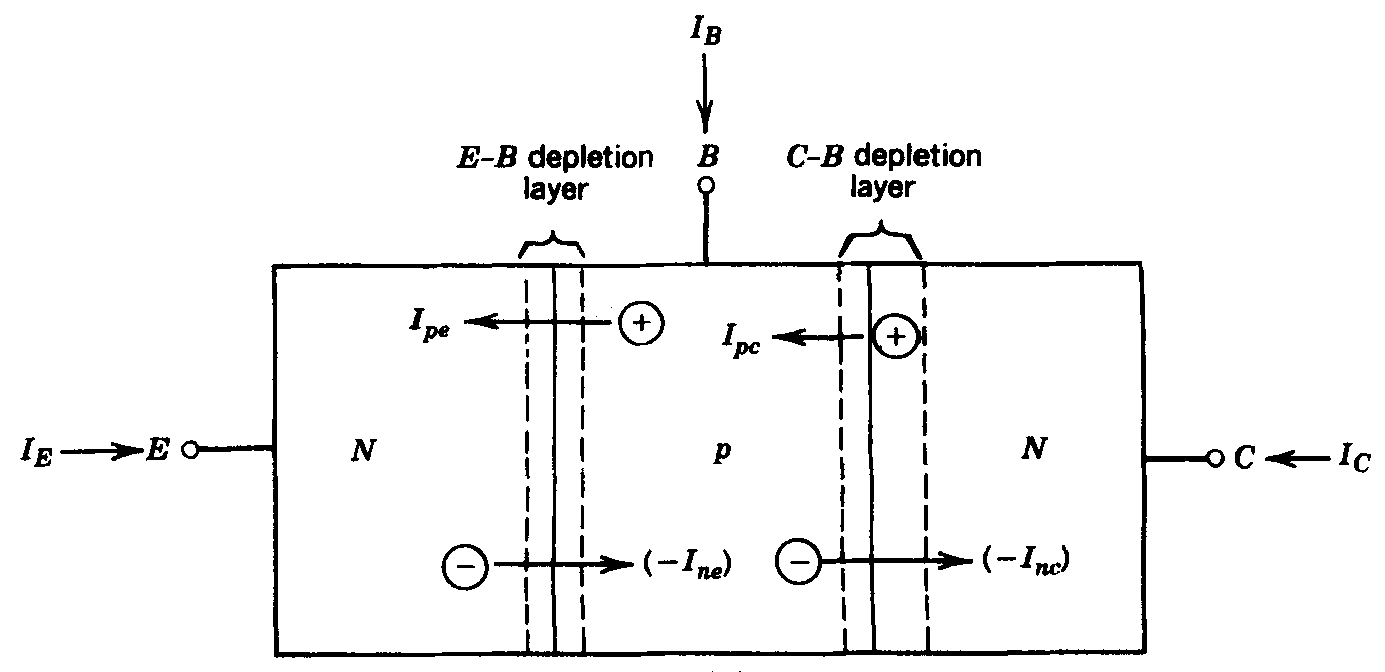
\includegraphics[width=1\textwidth]{fig/lec04/cross_section_BJT.png}
    \caption{Simplified cross-sectional model of BJT and current components; adapted from Ned Mohan, Tore M. Undeland, and William P. Robbins, Power Electronics: Converters, Applications, and Design, 3rd Edition.}
\end{figure}
\end{column}
\end{columns}
\end{frame}


\begin{frame}{\textbf{Diffusion Currents and Stored Charge Distribution}}
\begin{columns}
\begin{column}{0.6\textwidth}
\begin{itemize}
    \item The injected electrons from the emitter diffuse through the base to the collector, supported by the electric field across the reverse-biased base-collector junction.
    \item Recombination in the base is minimized due to short base width and high diffusion constant.
    \item Stored charge distribution within the base and collector regions affects dynamic response and switching.
    \item The base current includes three components:
    \begin{itemize}
        \item $I_{ne}$: diffusion of electrons injected from emitter to base.
        \item $I_{nc}$: recombination in the collector depletion layer.
        \item $I_{pe}$: holes injected into emitter to maintain charge neutrality.
    \end{itemize}
\end{itemize}
\end{column}

\begin{column}{0.4\textwidth}
\begin{figure}
    \centering
    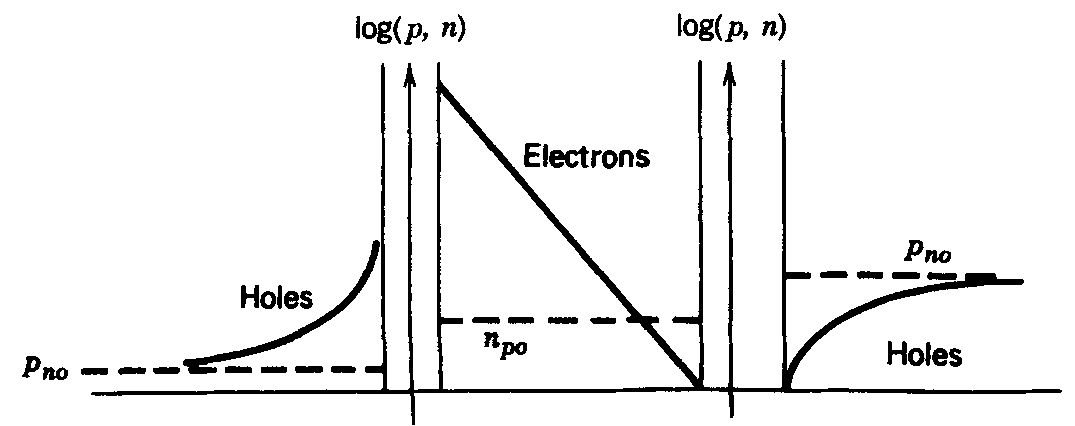
\includegraphics[width=1\textwidth]{fig/lec04/stored_charge_BJT.png}
    \caption{Stored charge vs. log(p,n) profile; adapted from Ned Mohan, Tore M. Undeland, and William P. Robbins, Power Electronics: Converters, Applications, and Design, 3rd Edition.}
\end{figure}
\end{column}
\end{columns}
\end{frame}


\begin{frame}{\textbf{Expression for Current Gain and Beta}}
    \begin{columns}
\begin{column}{0.65\textwidth}
\textbf{Terminal Current Definitions:}
\begin{equation}
\begin{aligned}
I_C &= I_{nc} \\
I_E &= I_{ne} + I_{pe} \\
I_B &= I_E - I_C = I_{ne} - I_{nc} + I_{pe}
\end{aligned}
\end{equation}
\textbf{Gain Expression:}
\begin{equation}
\frac{I_B}{I_C} = \frac{I_{ne} - I_{nc}}{I_{nc}} + \frac{I_{pe}}{I_{nc}} \Rightarrow \beta = \left( \frac{I_B}{I_C} \right)^{-1}
\end{equation}
\textbf{Optimization:}
\begin{itemize}
    \item Large $\beta$ requires: small $I_{pe}$ (via heavy emitter doping), minimal $(I_{ne} - I_{nc})$ (via long electron lifetime in base).
    \item Thin base to reduce recombination path and ensure efficient electron diffusion.
\end{itemize}
\end{column}

\begin{column}{0.35\textwidth}
\begin{figure}
    \centering
    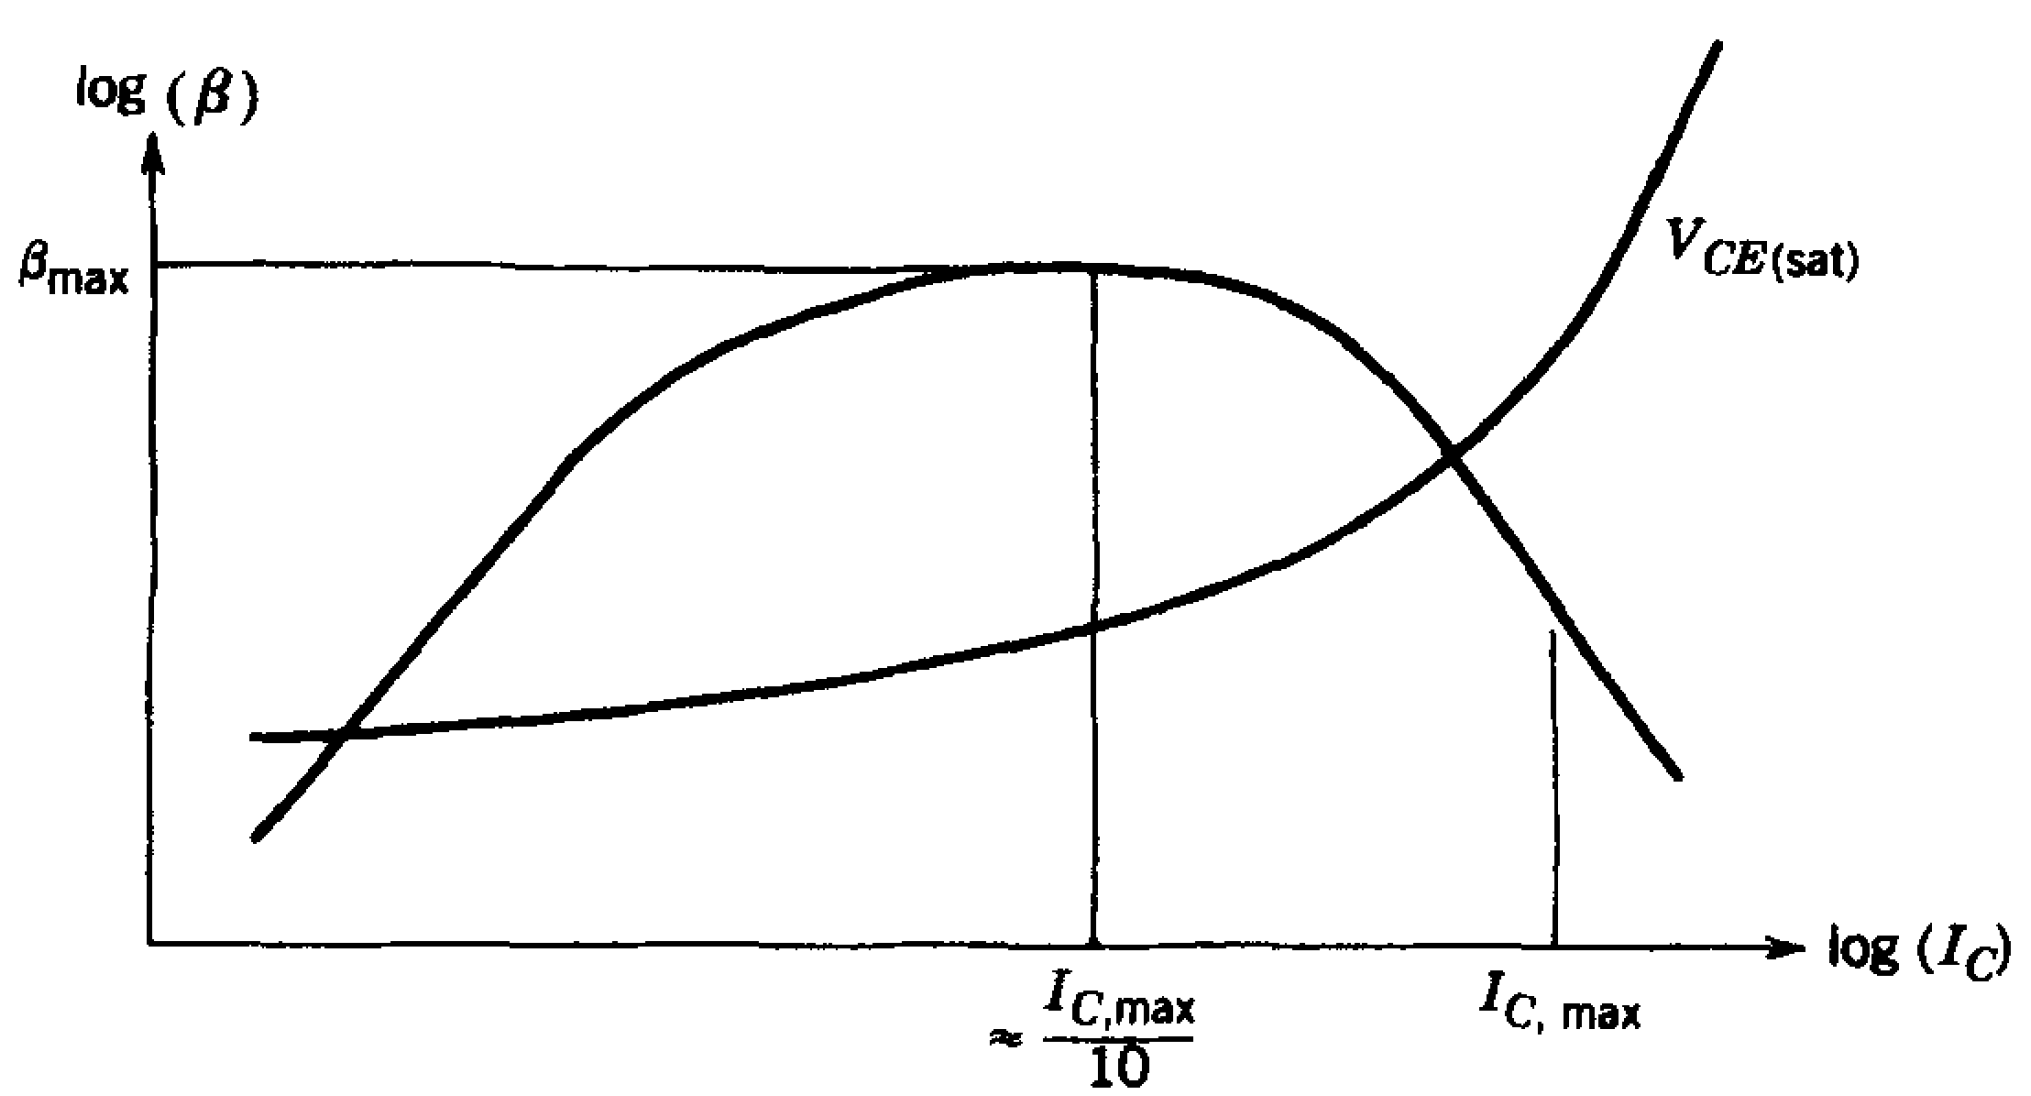
\includegraphics[width=1\textwidth]{fig/lec04/BJT_Current_gain_plot.png}
    \caption{Variation of BJT $\beta$ and $V_{CE(sat)}$, as a function of dc collector current; adapted from Ned Mohan, Tore M. Undeland, and William P. Robbins, Power Electronics: Converters, Applications, and Design, 3rd Edition.}
\end{figure}
\end{column}
\end{columns}
\end{frame}


\begin{frame}{\textbf{Emitter Current Crowding and its Impact on Beta}}
\begin{columns}
\begin{column}{0.6\textwidth}
\begin{itemize}
    \item Emitter current does not flow uniformly due to geometry and lateral resistance in the base.
    \item The voltage drop across the base-emitter junction is higher near the emitter edge, leading to current crowding.
    \item Result: Increased base current density at the emitter edge $\Rightarrow$ early onset of high-level injection $\Rightarrow$ fall in $\beta$.
    \item Modern power BJTs mitigate this by using interleaved emitter-base finger structures.
\end{itemize}
\end{column}

\begin{column}{0.4\textwidth}
\begin{figure}
    \centering
    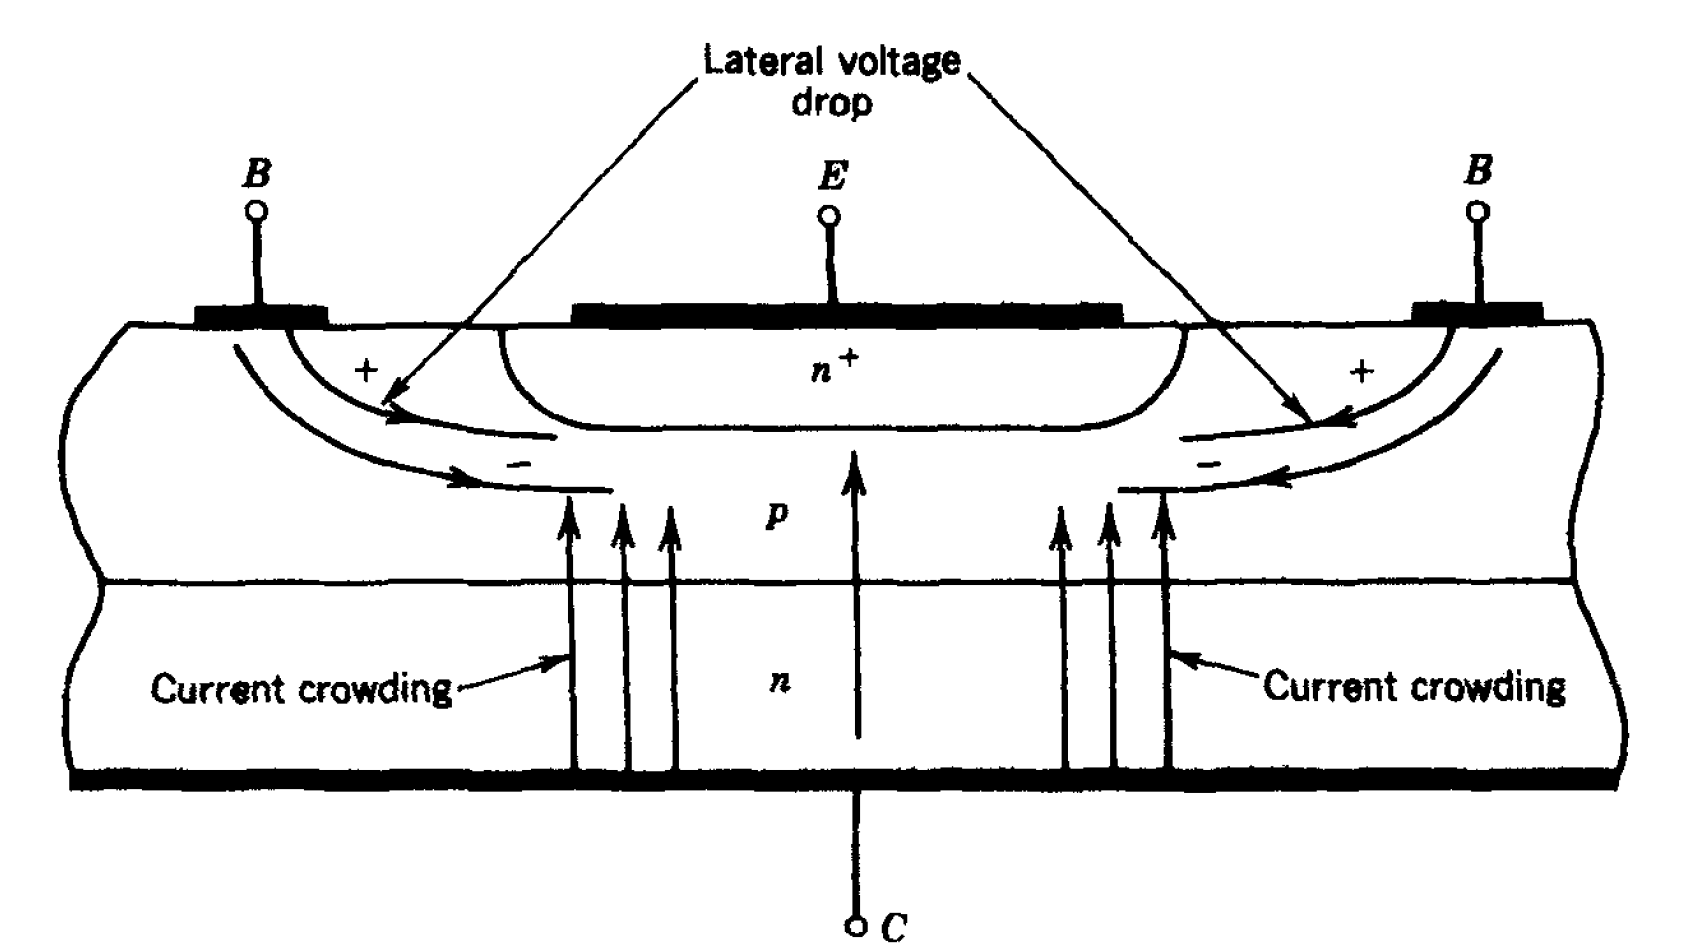
\includegraphics[width=0.6\textwidth]{fig/lec04/BJT_current_crowding.png}
    \caption{Forward-biased emitter current crowding due to lateral base resistance; adapted from Ned Mohan, Tore M. Undeland, and William P. Robbins, Power Electronics: Converters, Applications, and Design, 3rd Edition.}
\end{figure}
\end{column}
\end{columns}
\end{frame}


\begin{frame}{\textbf{Quasi-Saturation in Power BJTs}}
\begin{columns}
\begin{column}{0.55\textwidth}
\begin{itemize}
    \item At high $I_C$, the voltage drop across the drift region increases due to $R_d$.
    \item The base-collector junction becomes weakly forward biased.
    \item Hole injection from base to collector drift occurs, and space-charge neutrality requires electron injection as well.
    \item Drift region begins to accumulate charge on one side only — this is quasi-saturation.
\end{itemize}

\begin{equation}
i_C = \frac{V_{CE}}{R_d}
\end{equation}
\end{column}

\begin{column}{0.45\textwidth}
\begin{figure}
    \centering
    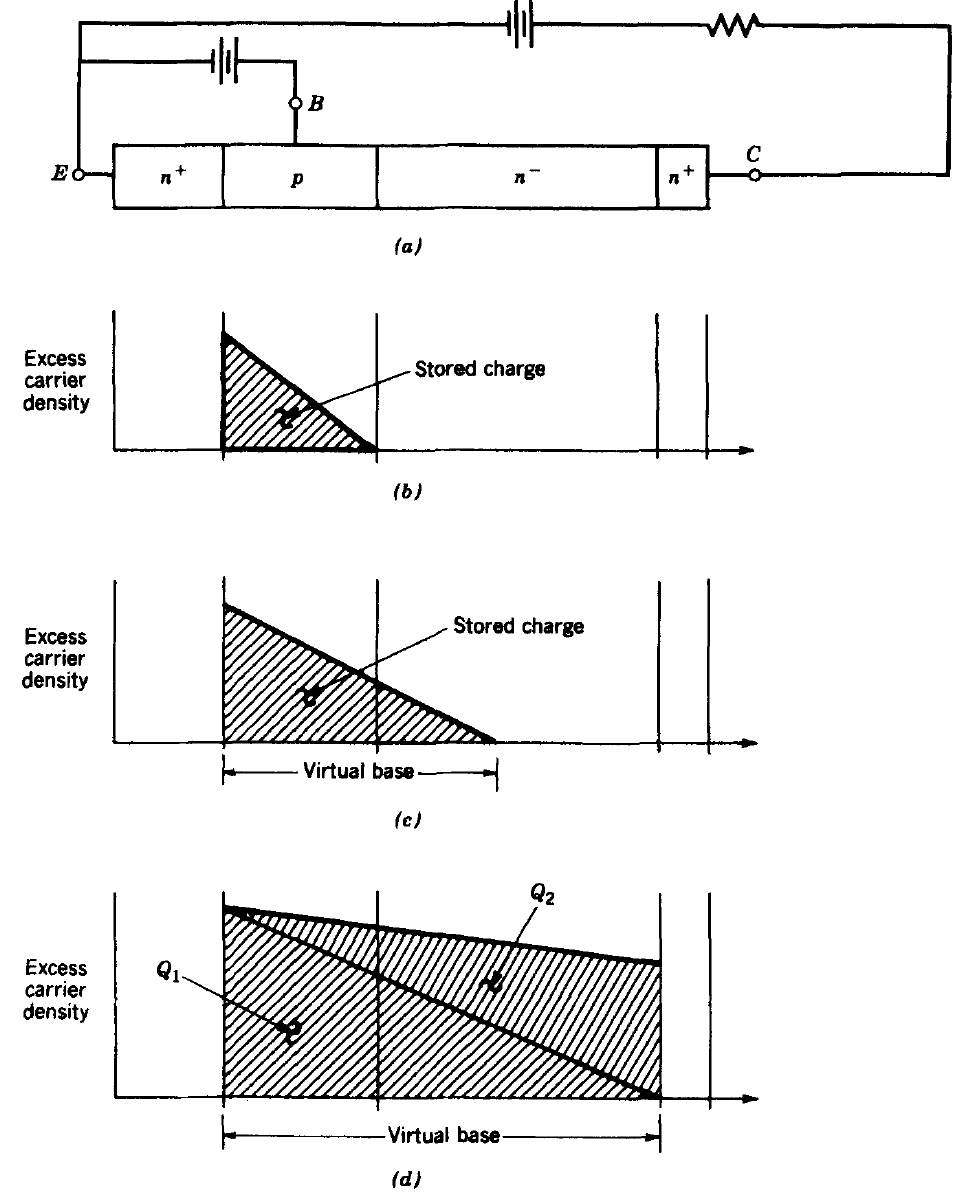
\includegraphics[width=0.5\textwidth]{fig/lec04/BJT_stored_charge_distribution.png}
    \caption{Charge profile showing virtual base in quasi-saturation; adapted from Ned Mohan, Tore M. Undeland, and William P. Robbins, Power Electronics: Converters, Applications, and Design, 3rd Edition.}
\end{figure}
\end{column}
\end{columns}
\end{frame}


\begin{frame}{Static Characteristics of BJT}
    \begin{columns}
    \begin{column}{0.55\textwidth}
    \begin{itemize}
        \item A BJT is a current-controlled device.
        \item Its output characteristic $i_C$ versus $V_{CE}$ depends on the base current $i_B$:
        \[
            i_C = f(V_{CE}, i_B)
        \]
        \item The collector current is ideally $i_C = \beta i_B$, where $\beta$ is the current gain of the transistor.
        \item However, due to the Early effect (modulation of base width with $V_{CE}$), $\beta$ is not constant.
        \item This leads to variation in $i_C$ for the same $i_B$ as $V_{CE}$ increases.
    \end{itemize}
    \end{column}

    \begin{column}{0.45\textwidth}
    \begin{figure}
        \centering
        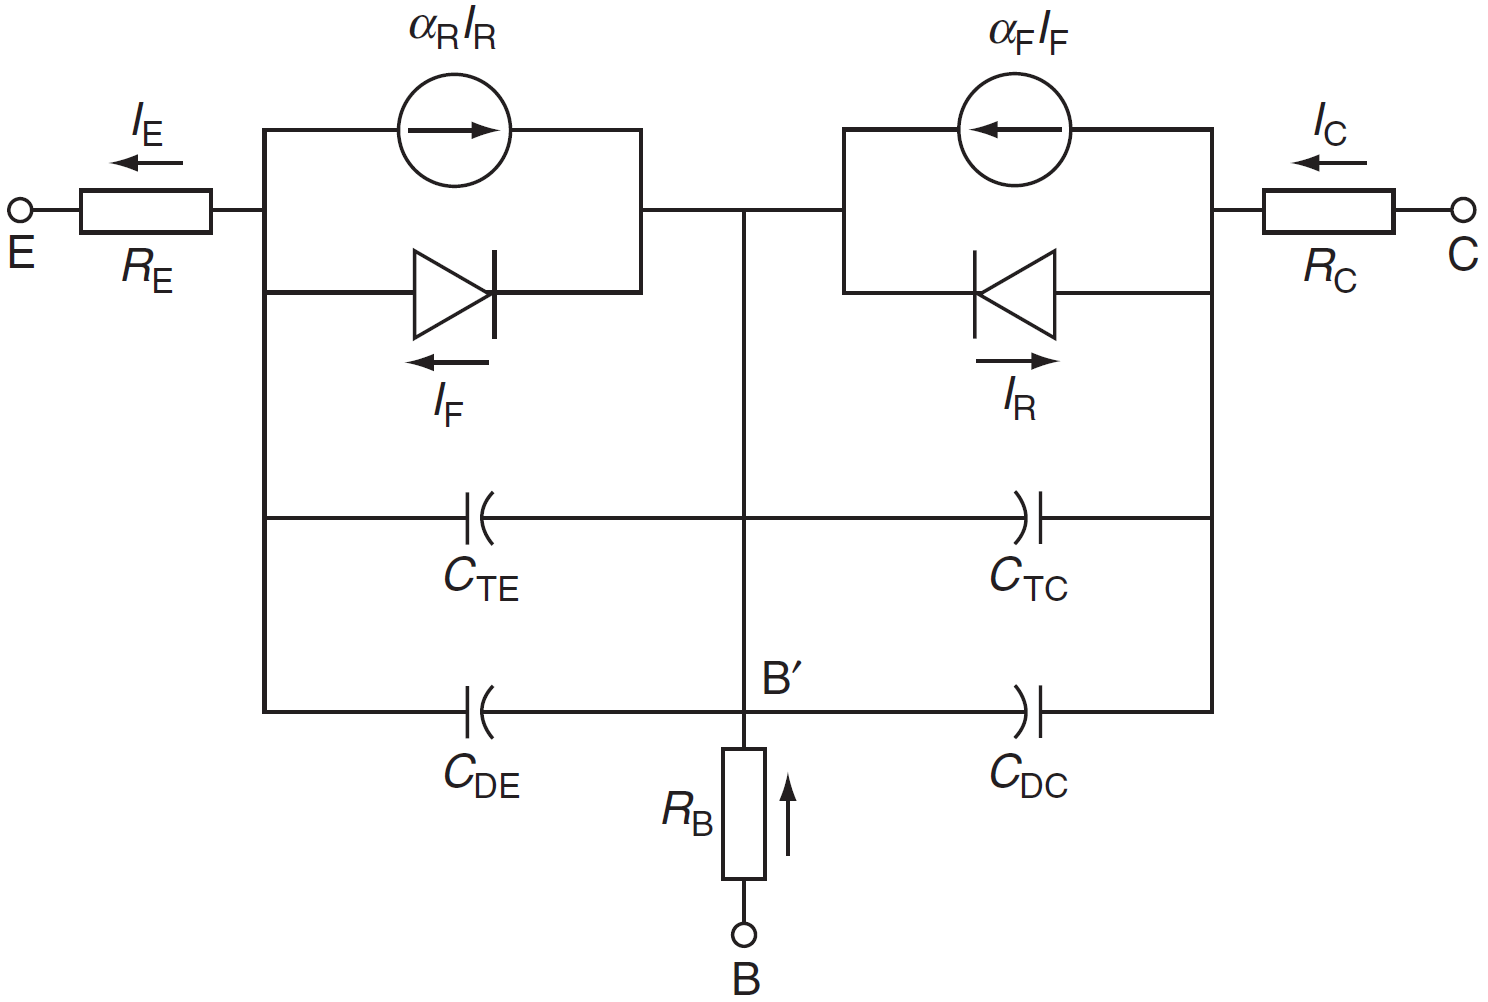
\includegraphics[width=1\textwidth]{fig/lec04/BJT_eq_circuit.png}
        \caption{BJT equivalent circuit with resistances and capacitances; ; adapted from Mohan et al., \textit{Power Electronics, 2nd Ed.}}
    \end{figure}
    \end{column}
\end{columns}
\end{frame}


\begin{frame}{Output Characteristics of a Transistor}
    \begin{columns}
    \begin{column}{0.55\textwidth}
    \begin{itemize}
        \item The $i_C$ vs $V_{CE}$ curve reveals three operating regions:
        \begin{enumerate}
            \item \textbf{Saturation Region:} Very low $V_{CE}$, high $i_C$, transistor fully ON.
            \item \textbf{Active Region:} $i_C \approx \beta i_B$, transistor used for amplification.
            \item \textbf{Cutoff Region:} $i_B \approx 0$, thus $i_C \approx 0$, transistor OFF.
        \end{enumerate}
        \item The Load Line on the output characteristic intersects the $i_C$-$V_{CE}$ curves based on $i_B$.
        \item Used to find the Q-point in analog design.
    \end{itemize}
    \end{column}

    \begin{column}{0.45\textwidth}
        \begin{figure}
        \centering
        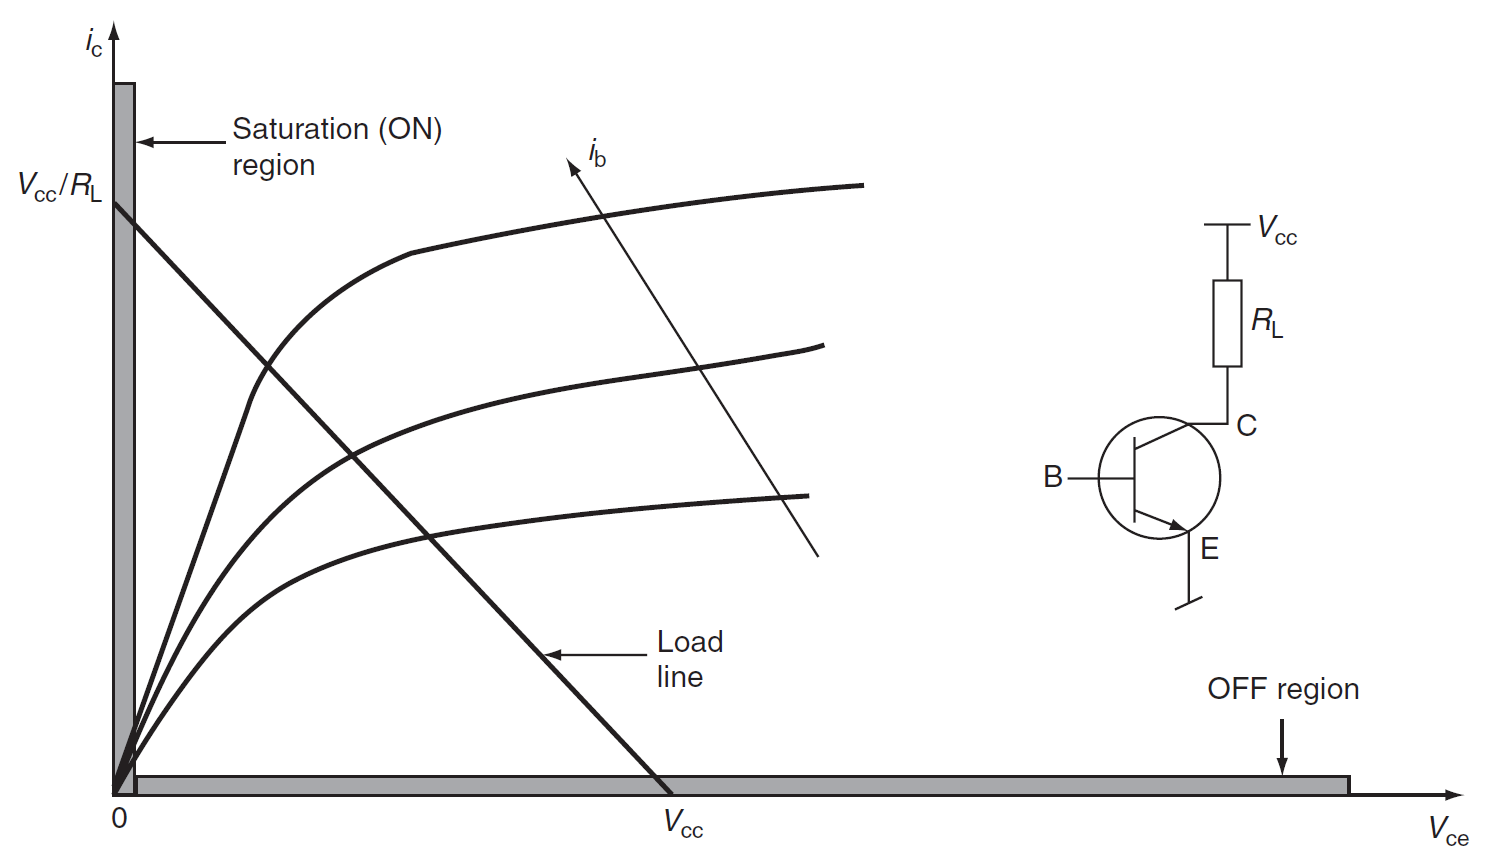
\includegraphics[width=1\textwidth]{fig/lec04/BJT_VI_Characteristics.png}
        \caption{Output characteristics of a BJT; adapted from Umanand, L., \textit{Power Electronics, Essentials and Applications.}}
    \end{figure}
    \end{column}
\end{columns}
\end{frame}


\begin{frame}{Power BJT – Static Characteristics}
    \begin{columns}
    \begin{column}{0.6\textwidth}

    \begin{itemize}
        \item Power BJTs exhibit similar $i_C$-$V_{CE}$ behavior but with effects like:
        \begin{itemize}
            \item \textbf{Quasi-saturation:} due to the lightly doped collector drift region.
            \item \textbf{Second breakdown:} due to localized thermal hotspots under high $i_C$.
        \end{itemize}
        \item Three major regions are:
        \begin{enumerate}
            \item Active region: Used for amplification.
            \item Quasi-saturation: Forward-biased $C$-$B$ junction begins to conduct.
            \item Hard saturation: Excess carrier injection across drift region.
        \end{enumerate}
        \item Breakdown voltages:
        \begin{itemize}
            \item $BV_{CBO}$: Collector-base with emitter open.
            \item $BV_{CEO}$: Collector-emitter with base open.
            \item $BV_{SUS}$: Sustaining voltage after breakdown onset.
        \end{itemize}
    \end{itemize}
    \end{column}

    \begin{column}{0.4\textwidth}
    \begin{figure}
        \centering
        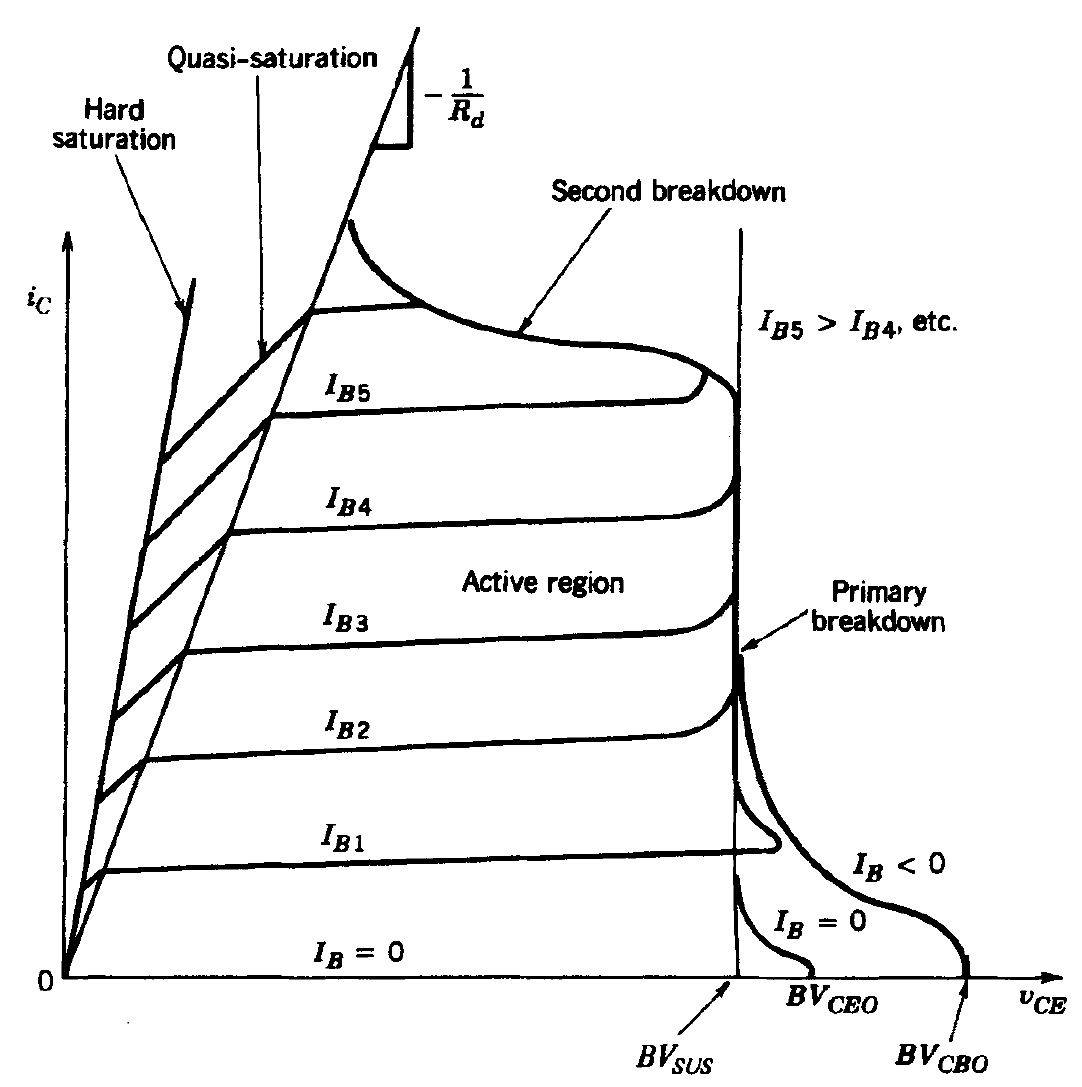
\includegraphics[width=0.8\textwidth]{fig/lec04/BJT_VI_Characteristics2.png}
        \caption{$i_C$-$V_{CE}$ curves with $I_B$ steps; adapted from Ned Mohan, Tore M. Undeland, and William P. Robbins, Power Electronics: Converters, Applications, and Design, 3rd Edition.}
    \end{figure}
    \end{column}
\end{columns}
\end{frame}

\begin{frame}{Current Gain and Load Line Intersection}
    \begin{columns}
    \begin{column}{0.6\textwidth}
    \begin{itemize}
        \item For a given $i_B$, collector current $i_C = \beta i_B$ in the active region.
        \item $\beta$ is affected by:
        \begin{itemize}
            \item Injection efficiency (related to emitter doping)
            \item Base transport factor (related to recombination and diffusion in base)
        \end{itemize}
        \item Load line defined by:
        \[
            i_C = \frac{V_{CC} - V_{CE}}{R_L}
        \]
        \item Intersection of load line and transistor characteristic determines Q-point.
    \end{itemize}
    \end{column}

    \begin{column}{0.4\textwidth}
    \begin{figure}
        \centering
        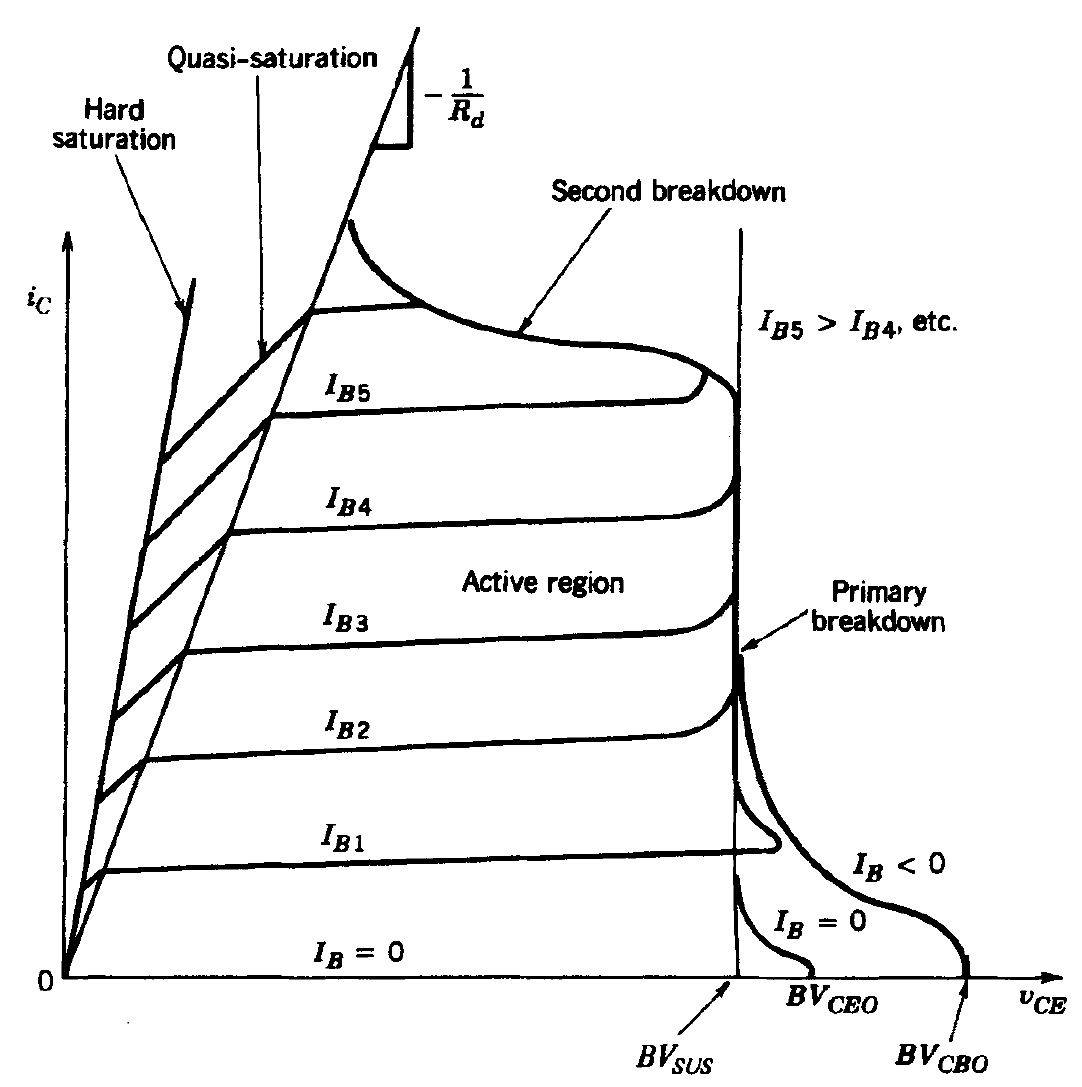
\includegraphics[width=0.8\textwidth]{fig/lec04/BJT_VI_Characteristics2.png}
        \caption{$i_C$-$V_{CE}$ curves with $I_B$ steps; adapted from Ned Mohan, Tore M. Undeland, and William P. Robbins, Power Electronics: Converters, Applications, and Design, 3rd Edition.}
    \end{figure}
    \end{column}
\end{columns}
\end{frame}


\begin{frame}{Key Observations in Power BJT Static Behavior}
    \begin{columns}
    \begin{column}{0.6\textwidth}
    \begin{itemize}
        \item Unlike small-signal BJTs, power BJTs show:
        \begin{itemize}
            \item \textbf{Lower current gain $\beta$}, especially in quasi-saturation.
            \item \textbf{Voltage fall-off due to second breakdown.}
            \item \textbf{Load line may enter second breakdown zone}, leading to thermal failure.
        \end{itemize}
        \item Quasi-saturation is due to double carrier injection in the collector drift region.
        \item Proper thermal and current limiting design is critical in power BJTs.
    \end{itemize}
    \end{column}

    \begin{column}{0.4\textwidth}
    \begin{figure}
        \centering
        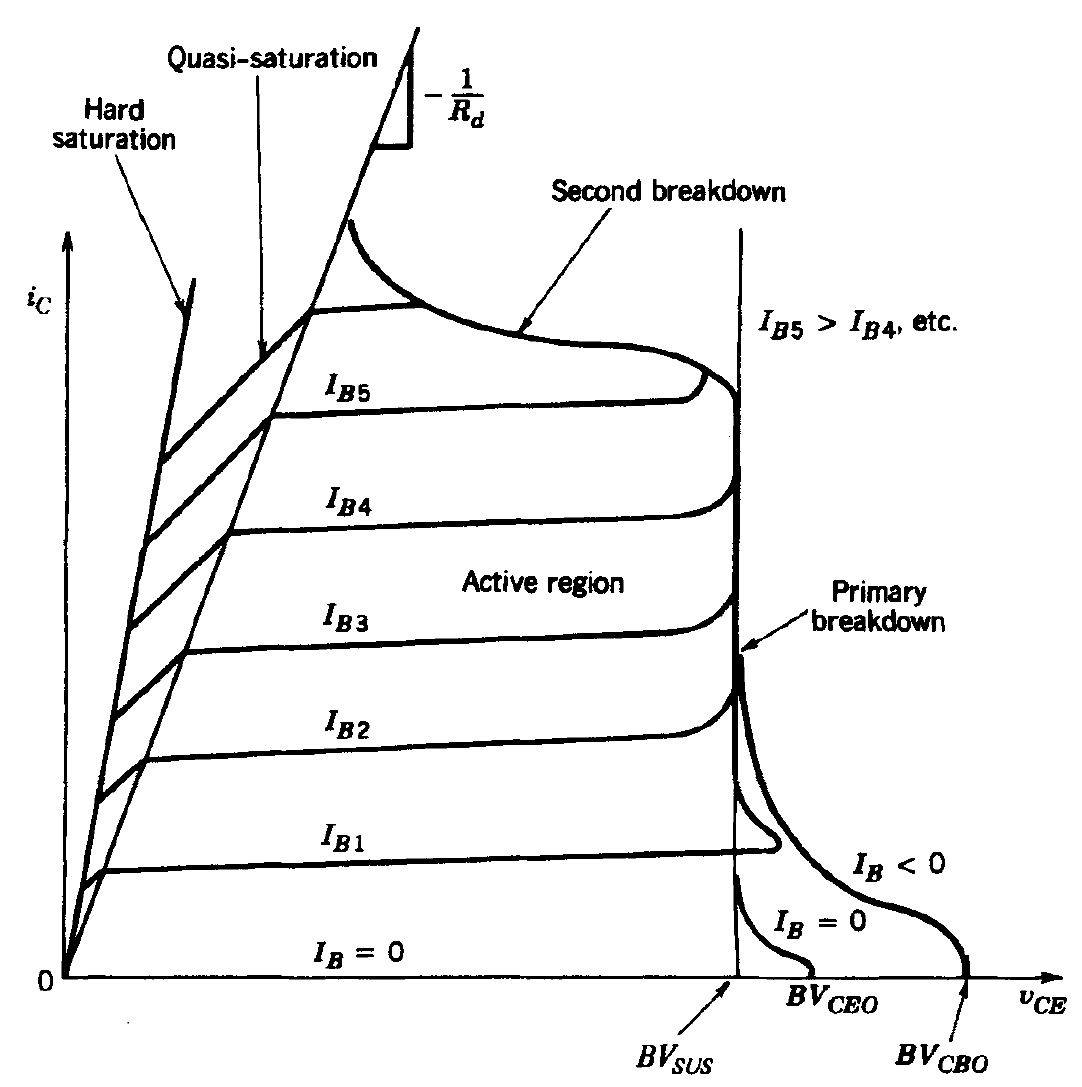
\includegraphics[width=0.8\textwidth]{fig/lec04/BJT_VI_Characteristics2.png}
        \caption{$i_C$-$V_{CE}$ curves with $I_B$ steps; adapted from Ned Mohan, Tore M. Undeland, and William P. Robbins, Power Electronics: Converters, Applications, and Design, 3rd Edition.}
    \end{figure}
    \end{column}
\end{columns}
\end{frame}



\begin{frame}{Dynamic Characteristics of BJT}
\textbf{In the ON-state, a transistor stores three main charges:}
\begin{enumerate}
    \item \textbf{$Q_b$}: Charge stored in the base region.
    \item \textbf{$Q_{ce}$}: Charge in the collector region beneath the emitter.
    \item \textbf{$Q_{cb}$}: Charge in the collector region beneath the base contact.
\end{enumerate}

\vspace{1em}
These charges define the transient behavior during switching. When transitioning to the OFF-state, all three must be removed for the transistor to fully block current.

\begin{figure}
    \centering
    % \includegraphics[width=0.7\linewidth]{your_figure_path}
    \caption{[Add diagram showing positions of $Q_b$, $Q_{ce}$, and $Q_{cb}$]}
\end{figure}
\end{frame}


\begin{frame}{Charge Dependency on $V_{CE}$ and $I_C$}
        \begin{columns}
    \begin{column}{0.5\textwidth}
\begin{itemize}
    \item \textbf{$Q_b$} is largely independent of $V_{CE}$, but increases with $I_C$.
    \item \textbf{$Q_{ce}$} increases with $I_C$ but decreases as $V_{CE}$ increases.
    \item \textbf{$Q_{cb}$} grows rapidly as $V_{CE}$ drops — marking the onset of saturation.
\end{itemize}

\textbf{Implication:} Charge buildup significantly affects collector-emitter voltage and switching speed.
    \end{column}

    \begin{column}{0.5\textwidth}
\begin{figure}
    \centering
    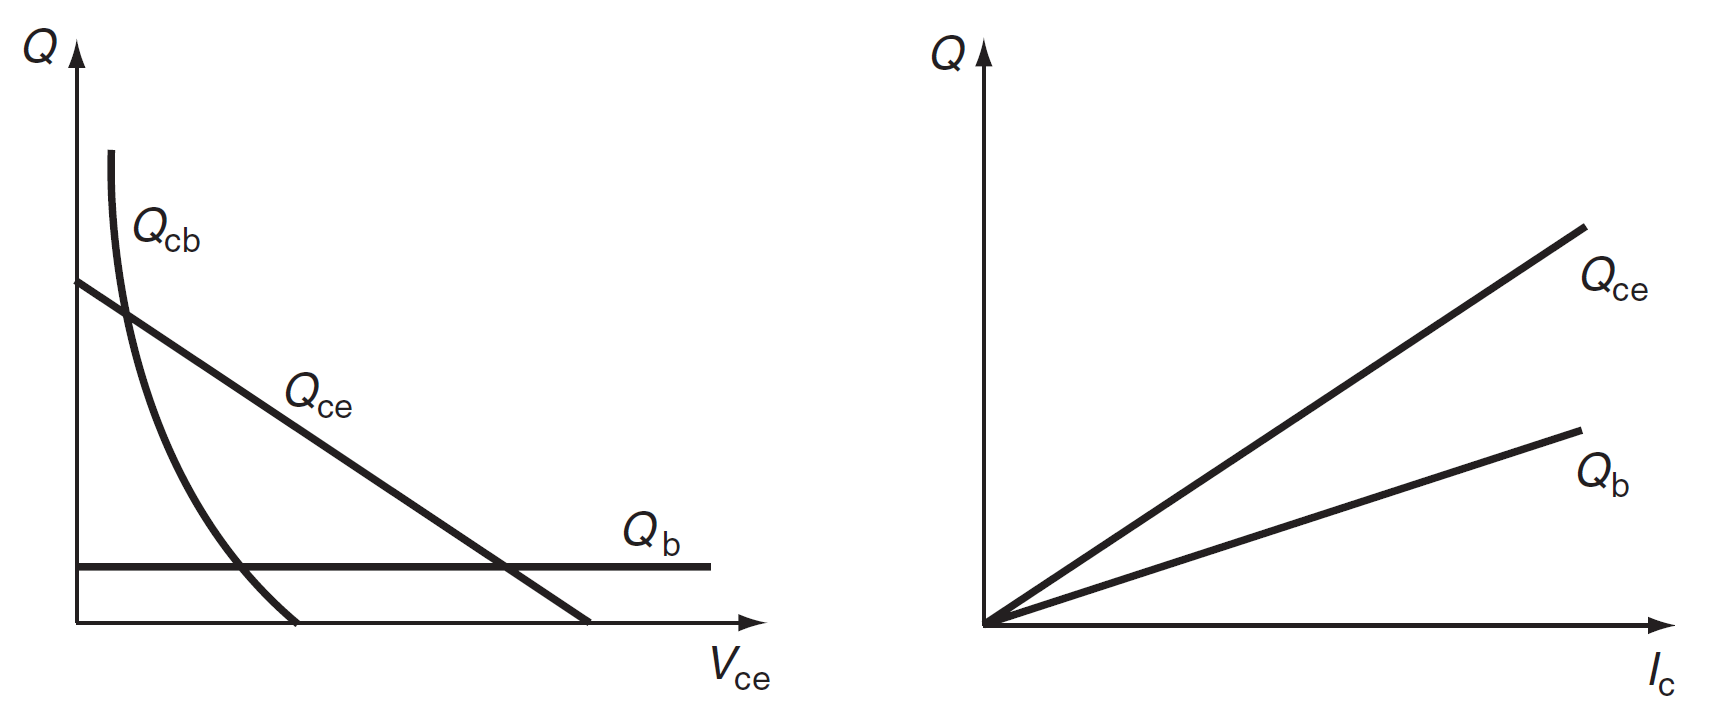
\includegraphics[width=1\linewidth]{fig/lec04/BJT_charge_dependancy.png}
    \caption{$Q$ vs $V_{CE}$ and $Q$ vs $I_C$; adapted from Umanand, L., \textit{Power Electronics, Essentials and Applications.}}
\end{figure}
    \end{column}
\end{columns}
\end{frame}


\begin{frame}{Turn-OFF of BJT – Physical Process}
  \begin{columns}
    \begin{column}{0.5\textwidth}
\begin{itemize}
    \item Turn-off begins when base drive is removed or reversed.
    \item $Q_b$ is removed first, starting from edges near the emitter.
    \item $Q_{ce}$ and $Q_{cb}$ follow, shrinking towards the center.
    \item Residual charge $Q_r$ creates a \textit{tail current}, affecting turn-off time.
\end{itemize}
\textbf{Storage time $t_s$}: Time during which current still flows due to residual charge even after base drive is removed.
    \end{column}

    \begin{column}{0.5\textwidth}
\begin{figure}
    \centering
    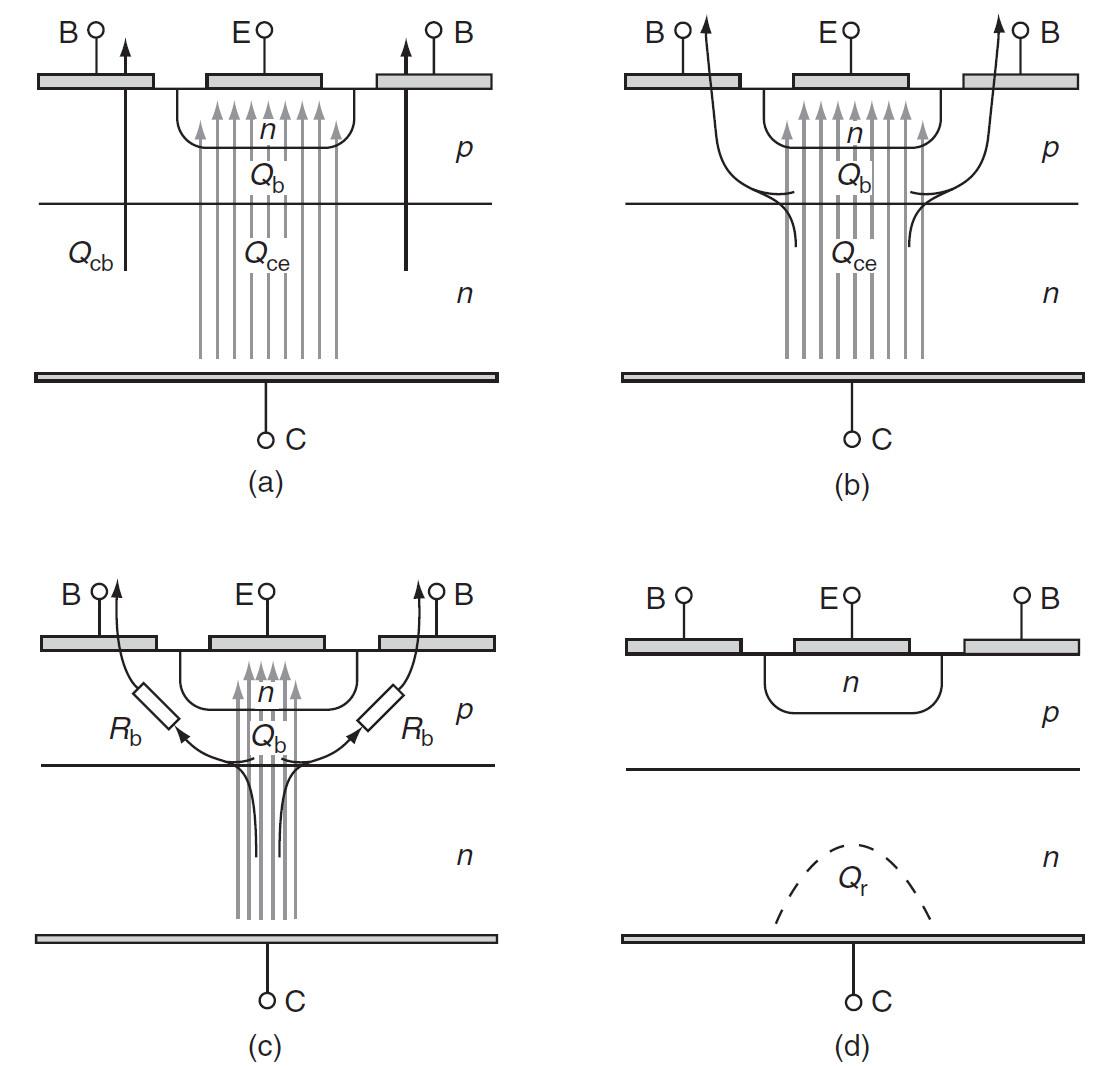
\includegraphics[width=0.65\linewidth]{fig/lec04/BJT_turn_off.png}
    \caption{BJT Turn-off process: charge removal sequence; adapted from Umanand, L., \textit{Power Electronics, Essentials and Applications.}}
\end{figure}
    \end{column}
\end{columns}
\end{frame}


\begin{frame}{Turn-ON of BJT – Dynamics}
  \begin{columns}
    \begin{column}{0.5\textwidth}
\begin{itemize}
    \item In OFF-state, there are no stored charges.
    \item A positive base pulse injects $Q_{ce}$, reducing $V_{CE}$ rapidly.
    \item A sharp peak in base current is ideal for quick charge buildup.
    \item Faster ON-switching means lower energy loss.
\end{itemize}

\textbf{Switching losses during turn-ON} depend on:
\begin{itemize}
    \item Time to establish $Q_{ce}$ and $Q_b$.
    \item Load characteristics (resistive or inductive).
\end{itemize}
    \end{column}

    \begin{column}{0.5\textwidth}
\begin{figure}
    \centering
    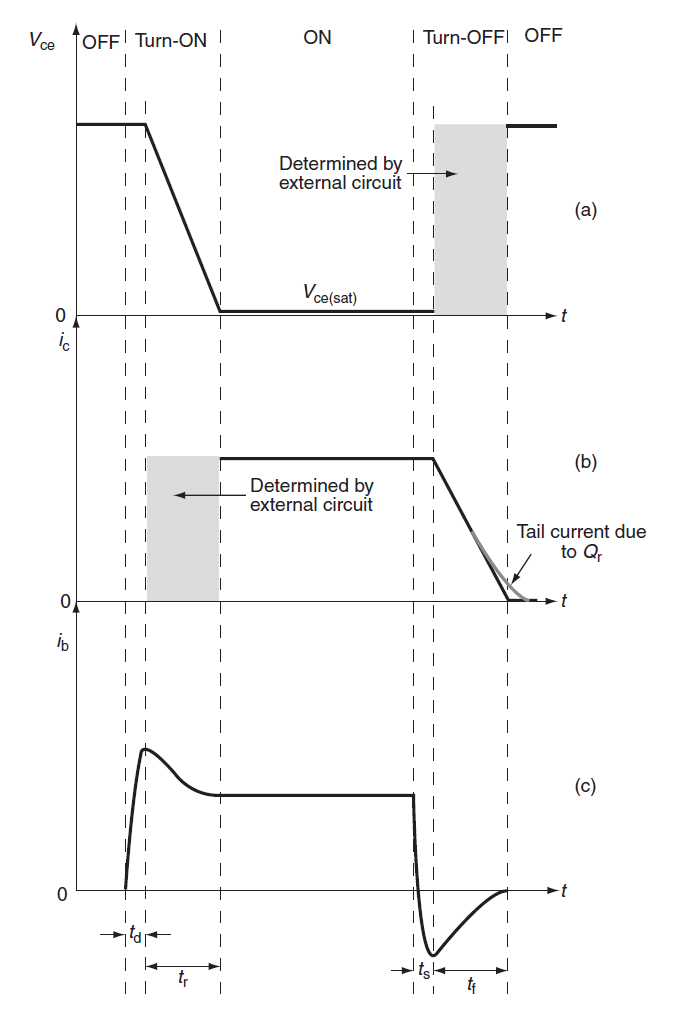
\includegraphics[width=0.5\linewidth]{fig/lec04/BJT_turn_on.png}
    \caption{BJT Turn-on process: charge buildup sequence; adapted from Umanand, L., \textit{Power Electronics, Essentials and Applications.}}
\end{figure}
    \end{column}
\end{columns}
\end{frame}



\begin{frame}{Power Dissipation in BJT}
\textbf{Total Power Dissipation:}
\[
P_d = P_{on} + P_{off} + P_{switching}
\]

\textbf{ON-state Loss:}
\[
P_{on} = V_{CE(sat)} \times I_C \times D
\]
where $D$ is the duty cycle.

\textbf{Switching Loss (OFF $\rightarrow$ ON):}
\[
P_{\text{OFF-ON}} = \frac{V_{cc} I_C t_f f_s}{6}
\]

\textbf{Switching Loss (ON $\rightarrow$ OFF):}
\[
P_{\text{ON-OFF}} = \frac{V_{cc} I_C t_r f_s}{6}
\]

\textbf{Total Switching Loss:}
\[
P_{\text{switching}} = \frac{V_{cc} I_C f_s (t_r + t_f)}{6}
\]
\end{frame}


\begin{frame}{Safe Operating Area (SOAR)}
      \begin{columns}
    \begin{column}{0.5\textwidth}
\textbf{SOAR}: Region where transistor operates safely under given voltage-current conditions.

\begin{itemize}
    \item Forward SOAR (FSOAR): With positive base drive.
    \item Reverse SOAR (RSOAR): With negative base drive (turn-off).
    \item Delimits power dissipation, collector voltage, and current density.
\end{itemize}

\textbf{Key Constraints:}
\begin{itemize}
    \item Second breakdown limit.
    \item Thermal limits (hot spot prevention).
    \item Switching-induced crowding.
\end{itemize}
    \end{column}

    \begin{column}{0.5\textwidth}
\begin{figure}
    \centering
    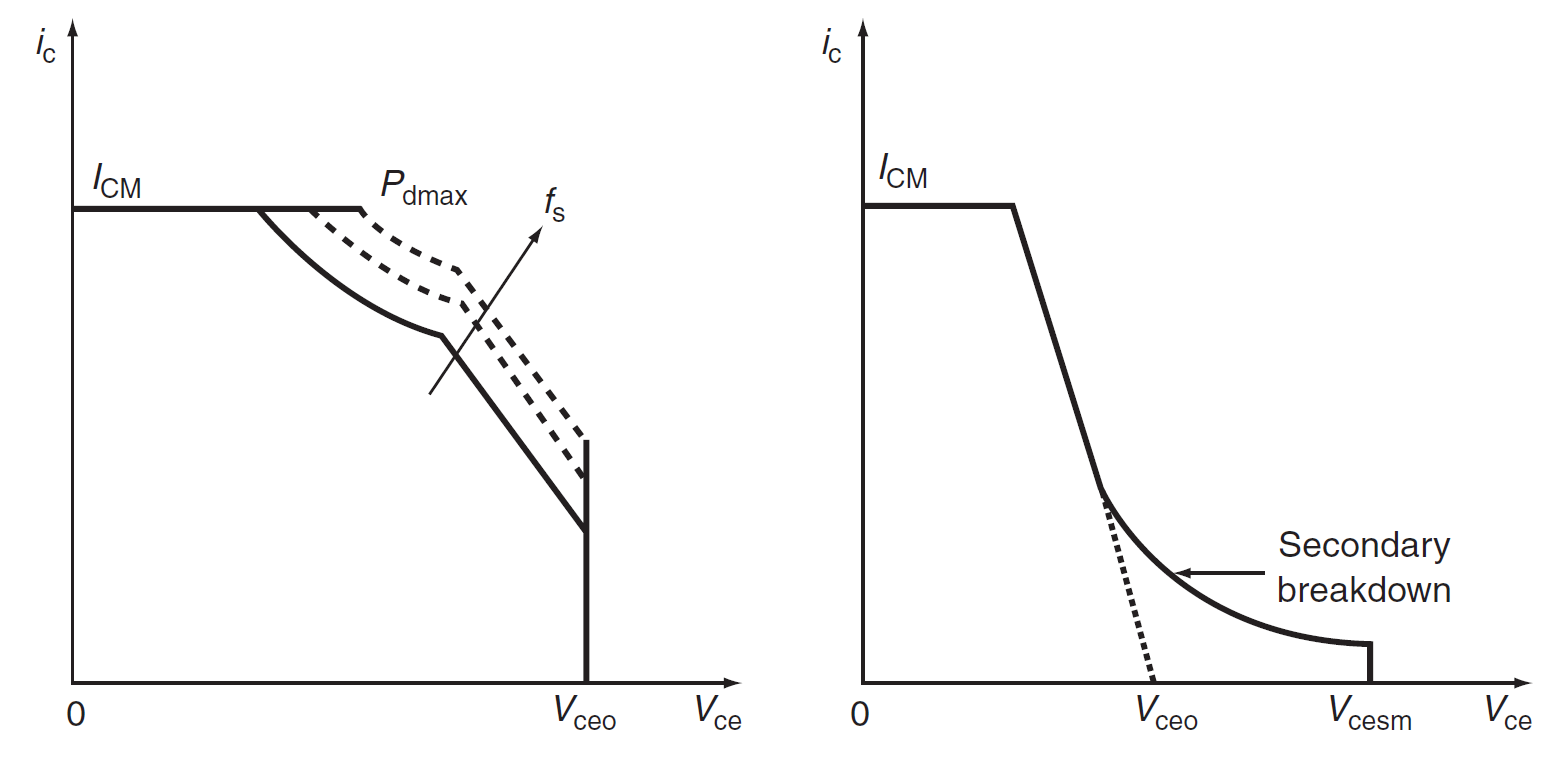
\includegraphics[width=0.8\linewidth]{fig/lec04/BJT_SOAR_RSOAR.png}
    \caption{SOAR and RSOAR curves for a power BJT; adapted from Umanand, L., \textit{Power Electronics, Essentials and Applications.}}
\end{figure}
    \end{column}
\end{columns}
\end{frame}


%------------------------------------------------

\begin{frame}{Breakdown Voltages in BJTs}
\begin{itemize}
  \item In the blocking state, the C--B junction must withstand the applied voltage.
  \item The B--E junction has a lower breakdown voltage (5–20 V) due to heavy emitter doping to achieve high $\beta$.
  \item To withstand high voltages, a lightly doped collector drift region is used.
  \item Base width is minimized to maintain gain but limited to avoid reach-through breakdown.
\end{itemize}
\vspace{0.5em}
\textbf{Design Trade-off:} Thin base for high gain vs. thick base for high voltage.
\textbf{Breakdown Voltage Expressions:}
\begin{itemize}
  \item In common-emitter configuration: $BV_{CEO} < BV_{CBO}$
  \item Relationship:
  \[
  BV_{CEO} = \frac{BV_{CBO}}{\beta^{1/n}} \quad \text{where } n = 4 \text{ for } npn, n = 6 \text{ for } pnp
  \]
  \item Due to reverse-bias current $I_{CBO}$ at B--E junction, impact ionization rate increases in emitter-open mode.
\end{itemize}
\end{frame}

%------------------------------------------------

\begin{frame}{Second Breakdown, Thermal Runaway and Localized Hotspots}
\begin{itemize}
  \item Occurs at high $V_{CE}$ and $I_C$ despite staying below primary breakdown.
  \item Triggered by localized thermal runaway and current filamentation.
  \item Exponential increase in power dissipation with temperature due to:
  \[
  n_i \propto \exp\left(-\frac{E_g}{2kT}\right)
  \]
  \item Dangerous due to steep $V_{CE}$ drop and rapid localized heating.
\end{itemize}
\textbf{Thermal Runaway and Localized Hotspots}
\begin{itemize}
  \item Filamentation: nonuniform current density leads to $J_A > J_B$
  \item Result: $T_A > T_B$ $\Rightarrow$ runaway due to positive feedback
  \item Region A may exceed intrinsic temperature $T_i$ causing catastrophic failure.
  \item Preventive measures:
  \begin{itemize}
    \item Use of snubbers and freewheeling diodes.
    \item Narrow emitter stripes.
    \item Controlled $di/dt$ and $dv/dt$ during switching.
  \end{itemize}
\end{itemize}
\end{frame}

%------------------------------------------------

\begin{frame}{On-State Losses}
    \begin{columns}
        \begin{column}{0.5\textwidth}
            \begin{itemize}
                \item Dominated by conduction loss:
                \[
                P_{on} = I_C \cdot V_{CE(sat)}
                \]
                \item $V_{CE(sat)}$ increases with $I_C$ due to:
                \[
                V_{CE(sat)} = V_{BE(on)} - V_{BC(sat)} + V_d + I_C(R_e + R_c)
                \]
                \item Main contributor: $V_d$ across collector drift region.
                \item $V_d$ depends on carrier lifetime; trade-off between low $V_d$ and fast switching.
            \end{itemize}
        \end{column}

\begin{column}{0.5\textwidth}
\begin{figure}
\centering
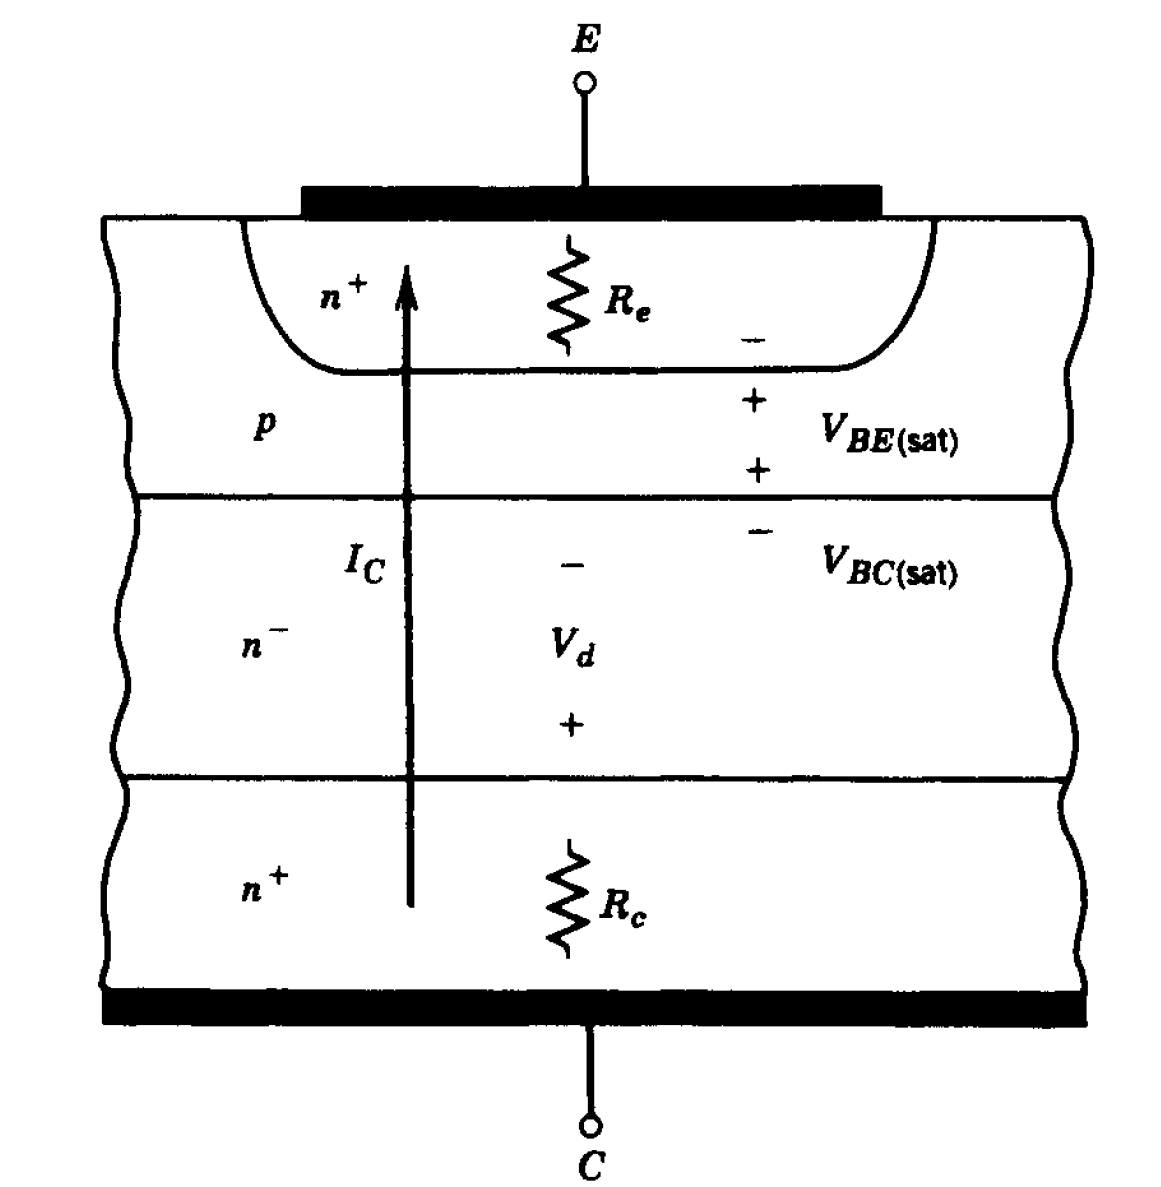
\includegraphics[width=0.6\textwidth]{fig/lec04/BJT_on_state_losses.png}
\caption{On-state losses in a BJT; adapted from Umanand, L., \textit{Power Electronics, Essentials and Applications.}}
\label{fig:bjt_on_state_losses}
\end{figure}
    \end{column}
    \end{columns}
\end{frame}

%------------------------------------------------

\begin{frame}{Paralleling of BJTs}
        \begin{columns}
        \begin{column}{0.5\textwidth}
\begin{itemize}
  \item Used in high-current applications to share load.
  \item Risk: thermal runaway due to negative temp. coeff. of $V_{BE}$.
  \item Solution: Add emitter resistance $R$ for negative feedback.
  \[
  V_{be1} = V_{be2} + R(I_{c1} - I_{c2}) \Rightarrow \Delta V_{be} = R \Delta I_c
  \]
  \item Limit $\Delta V_{be}$ to $\approx$ 0.2 V to allow $\Delta I_C \leq 0.5$ A.
\end{itemize}
        \end{column}

\begin{column}{0.5\textwidth}
\begin{figure}
\centering
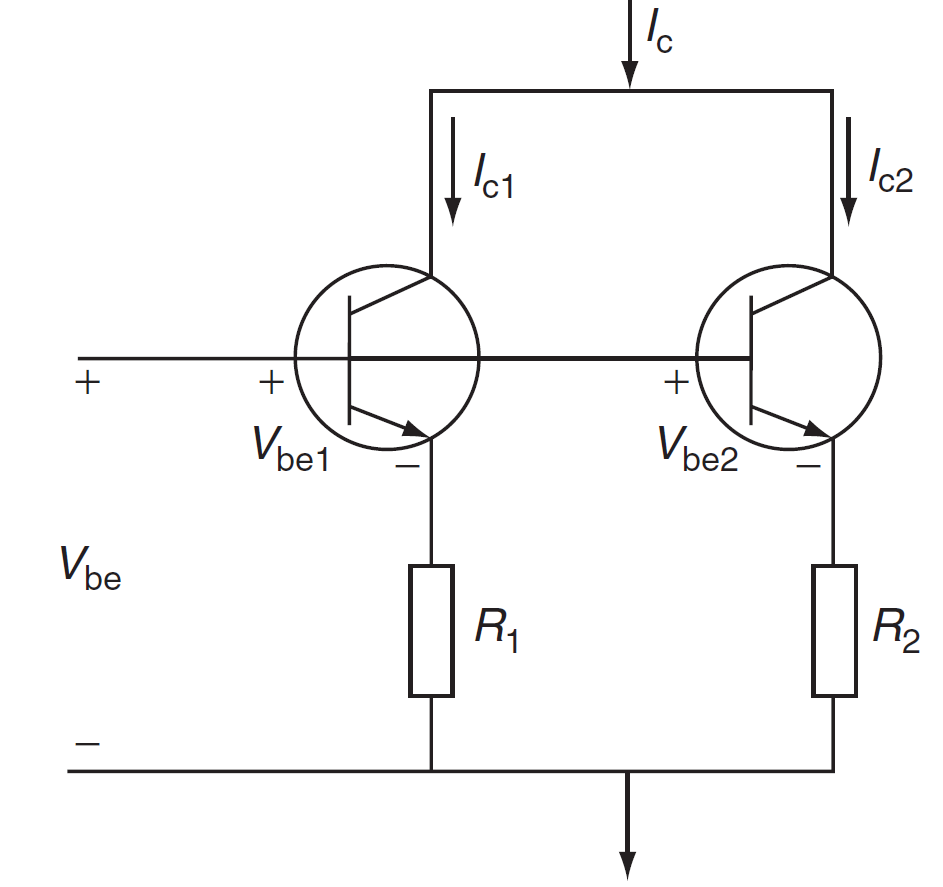
\includegraphics[width=0.6\textwidth]{fig/lec04/BJT_parallel.png}
\caption{Paralleling of BJT; adapted from Umanand, L., \textit{Power Electronics, Essentials and Applications.}}
\label{fig:bjt_on_state_losses}
\end{figure}
    \end{column}
    \end{columns}
\end{frame}

%------------------------------------------------

\begin{frame}{Darlington Connection}
            \begin{columns}
        \begin{column}{0.5\textwidth}
\begin{itemize}
  \item Used to boost current gain:
  \[
  I_B = \frac{I_C}{\beta_1 \cdot \beta_2}
  \]
  \item Higher $V_{CE(sat)} \approx$ 1–1.2 V compared to 0.4–0.6 V for single BJT.
  \item Ideal for high-power applications where base drive must be minimized.
  \item Trade-off: higher power loss and slower switching.
\end{itemize}
        \end{column}

\begin{column}{0.5\textwidth}
\begin{figure}
\centering
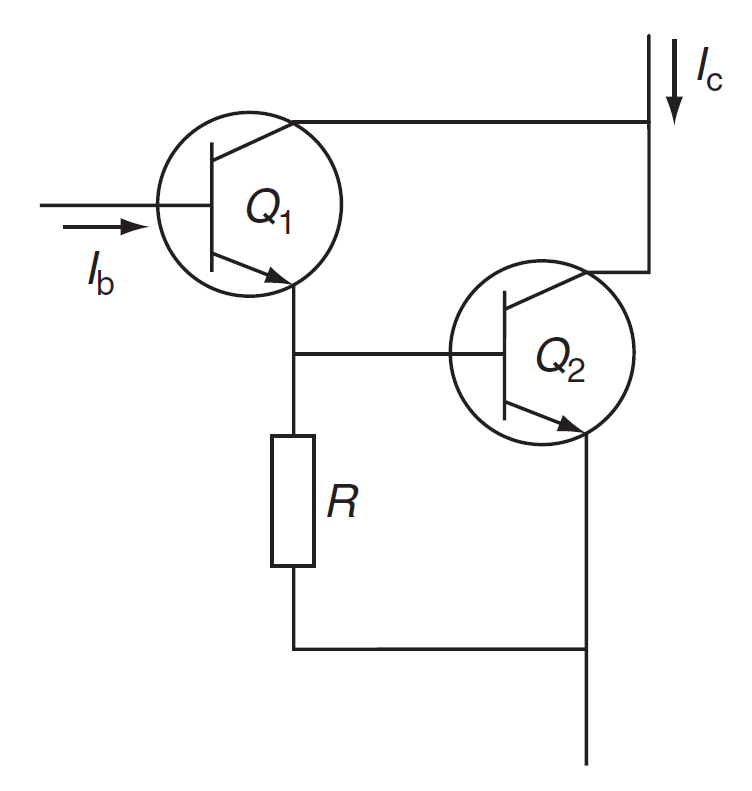
\includegraphics[width=0.6\textwidth]{fig/lec04/darlington_BJTs.png}
\caption{Darlington; adapted from Umanand, L., \textit{Power Electronics, Essentials and Applications.}}
\label{fig:bjt_on_state_losses}
\end{figure}
    \end{column}
    \end{columns}
\end{frame}